%BAB_3 LAPORAN KP

\chapter{PERANCANGAN SISTEM}
Pada bab ini akan disajikan mekanisme perancangan alat, baik perangkat keras ataupun perangkat lunak untuk mewujudkan sebuah robot lengan. Tahapan perancangan dimulai dari perancangan diagram blok sistem, perancangan perangkat keras, perancangan perangat lunak, perancangan kinematika balik, perancangan GUI, dan integrasi keseluruhan program. 
\section{ Diagram Blok Sistem }
Secara garis besar pada tahapan implementasi dari kinematika pada \textit{arm manipulator robot} SCARA ini menggunakan \textit{output} atau penggerak berupa motor DC dengan \textit{feedback} posisi berupa \textit{potensiometer} sedangkan pada bagian  \textit{input} yang berasal dari GUI yang dibuat pada Processing IDE mengirimkan sebuah koordinat yang digunakan untuk menentukan pergerakan robot berdasarkan fungsi \textit{inverse kinematic}. Gambar \ref{pic.diagram.bloksistem} merupakan diagram blok sistem secara keseluruhan.
\begin{figure}[H]
	\centering
	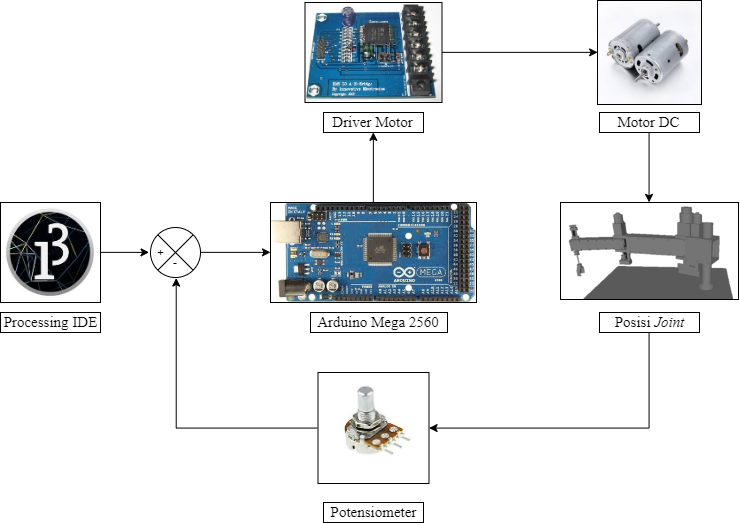
\includegraphics[width=13cm]{gambar/Rangkaian_Diagram.png}
	\caption{Diagram Blok Sistem}
	\label{pic.diagram.bloksistem}
\end{figure}
Pada blok diagram yang disajikan pada Gambar \ref{pic.diagram.bloksistem} sistem terdiri dari bagian – bagian yang meliputi bagian masukan, bagian kendali, bagian keluaran, dan bagian penampil. Pada bagian masukan menggunakan GUI yang dirancang pada Processing IDE yang digunakan sebagai \textit{forward kinematic} serta \textit{inverse kinematic} dimana robot akan bergerak menyesuaikan dengan posisi atau sudut yang diinputkan melauli Processing IDE. 
Pada bagian kontrol menggunakan Arduino Mega 2560 sebagai mikrokontroler yang mengendalikan seluruh operasi dari robot. \textit{Power supply} Arduino sebesar 5 volt DC didapatkan dari regulator tegangan yang menurunkan tegangan dari 24 volt DC ke 5 volt DC. 

Pada bagian keluaran, pin \textit{Pulse With Modulation} (PWM) pada Arduino Mega 2560 dihubungkan dengan \textit{driver} motor yang digunakan untuk mengontrol arah pergerakan dari motor DC serta kecepatan pergerakan dari motor DC. Pergerakan arah putaran motor DC bergantung pada \textit{feedback} posisi setiap sendi yang diberikan oleh \textit{potensiometer}. Tiga buah pin digital ardunio dihubungkan pada rangkaian \textit{switch} yang menggunakan IC TIP31 yang berfungsi sebagai kontrol dari \textit{End-Effector} yang dioperasikan menggunakan tekanan udara yang dikontrol oleh \textit{valve pneumatic.}

Pada bagian penampil merupakan bentuk dari rancangan GUI yang dirancang dalam Processing IDE melalui sebuah bentuk pemrograman. Dalam tampilan GUI terdapat beberapa \textit{tools} yang dapat untuk mengatur pergerakan robot SCARA. Pada GUI menampilkan nilai dari sudut, dan posisi serta animasi robot SCARA pada kondisi langsung dari pergerakan robot SCARA.
\section{ Perancangan Perangkat Keras }
Perancangan perangkat keras pada \textit{arm manipulator robot} SCARA terdiri dari dua bagian yaitu bagian mekanis dan elektronis. Bagian  mekanis merupakan bagian \textit{hardware} yang meliputi desain, bahan dan bentuk dari\textit{ arm manipulator robot} SCARA. Bagian elektronis merupakan bagian \textit{hardware} yang meliputi sistem – sistem yang berkaitan dengan rangkaian pada robot SCARA seperti rangkaian pada desain \textit{board} serta komponen – komponen elektronis pendukung.
\subsection{ Sistem Mekanis }
Sistem mekanika dari robot lengan bergantung dari konfigurasi robot lengan. Konfigurasi robot lengan terbagi menjadi enam, yaitu konfigurasi \textit{Articulated}, konfigurasi SCARA, konfigurasi \textit{Spherical}, konfigurasi \textit{Cylindrical}, dan konfigurasi \textit{Cartesian}. Pada Kerja Praktik ini konfigurasi robot lengan yang digunakan adalah konfigurasi SCARA dengan dua \textit{joint} \textit{revolute} dan satu \textit{end-effector}. Sistem mekanik dari lengan robot tiga DOF sangat berpengaruh dan mendominasi sistem karena bentuk dan pergerakan dari mekanik akan mempengaruhi elektronis serta program. Sistem mekanik yang baik sangat mendukung dari pergerakan robot, oleh karena itu perancangan mekanik harus proporsional dari panjang setiap lengan, lebar serta tinggi robot. Gambar \ref{pic.freebodyscara} merupakan \textit{free body} dari robot SCARA. Gambar \ref{pic.fisikscara} merupakan bentuk fisik dari robot SCARA yang digunakan pada penelitian kali ini.
\begin{figure}[H]
	\centering
	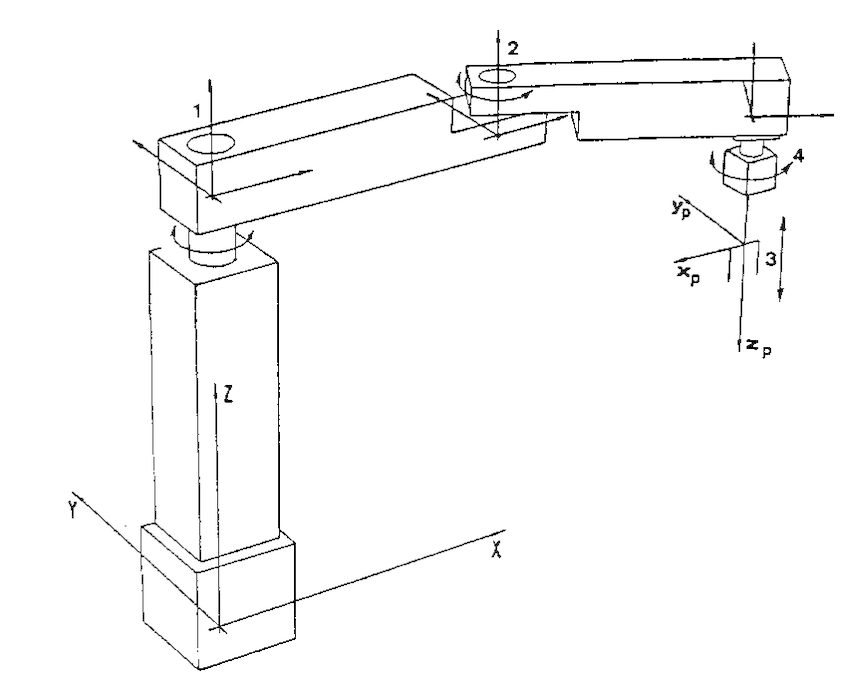
\includegraphics[width=7cm]{gambar/scaraa.png}
	\caption{\textit{Free Body} Robot SCARA}
	\label{pic.freebodyscara}
\end{figure}
\begin{figure}[H]
	\centering
	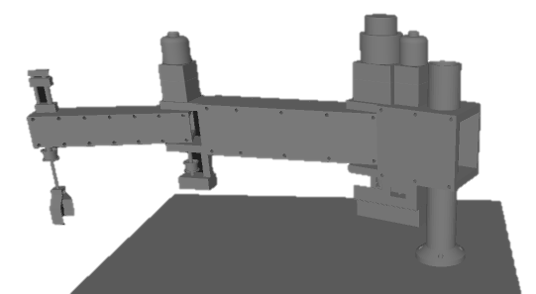
\includegraphics[width=7cm]{gambar/3dscara.png}
	\caption{Bentuk Fisik Robot SCARA}
	\label{pic.fisikscara}
\end{figure}
Robot SCARA merupakan robot yang meiliki tiga buah derajar kebebasan (DOF) yang terletak pada \textit{shoulder}, \textit{elbow}, dan pada \textit{end-effector}. Seluruh derajat kebebasan menggunakan sebuah motor DC yang didalamnya terdapat\textit{ gear box} untuk motor DC yang ada pada \textit{shoulder} dan \textit{elbow} untuk melakukan pergerakan. Sedangkan motor DC pada \textit{end-effector} dibantu oleh sebuah \textit{belt} untuk menyalurkan putaran dari motor yang terletak pada \textit{shoulder}. Pergerakan pada masing-masing \textit{joint} memiliki jangkauan maksimum yang berbeda-beda. Jangkauan juga dipengaruhi oleh panjangnya lengan yang dimiliki oleh robot SCARA tersebut. Tabel \ref{tbl.spesifikasiscara} merupakan spesifikasi dari robot SCARA yang digunakan.

\begin{table}[h]
		\centering
	\caption{Spesifikasi Robot SCARA}
	\label{tbl.spesifikasiscara}
	\begin{tabular}{|c|l|l|}
		\hline
		\rowcolor[HTML]{9B9B9B} 
		No & \multicolumn{1}{c|}{\cellcolor[HTML]{9B9B9B}Keterangan} & \multicolumn{1}{c|}{\cellcolor[HTML]{9B9B9B}Nilai} \\ \hline
		1  & \cellcolor[HTML]{FFFFFF}Main arm length                 & \cellcolor[HTML]{FFFFFF}360 mm                     \\ \hline
		2  & Fore arm length                                         & 290 mm                                             \\ \hline
		3  & Shoulder movement                                       & 180 °                                              \\ \hline
		4  & Elbow movement                                          & 200 °                                              \\ \hline
		5  & Wrist rotation                                          & 360 °                                              \\ \hline
		6  & Up \& down movement                                     & 150 mm                                             \\ \hline
		7  & Maximum tip velocity                                    & 3.0 kg                                             \\ \hline
	\end{tabular}
\end{table}
Desain pada\textit{ arm manipulator robot} SCARA berbahan besi dengan tebal 2 mm dengan tiga derajat kebebasan yang meliputi bagian \textit{shoulder}, \textit{elbow} serta \textit{end-effector}. Desain robot SCARA terbagi menjadi dua bagian. Bagian utama adalah \textit{box} panel yang berisi sistem elektronis utama dan pada bagian yang lain merupakan lengan dari robot SCARA sendiri. Terdapat juga tiga buah saluran udara yang berfungsi untuk mentransformasikan tekanan udara untuk pergerakan vertikal dari \textit{end-effector} yang berasal dari sebuah kompresor.  Dalam komunikasinya dengan komputer personal, robot SCARA dihubungkan dengan konektor USB. Gambar \ref{pic.boxpanel} merupakan bentuk fisik dari box panel pada Robot SCARA.
\begin{figure}[H]
	\centering
	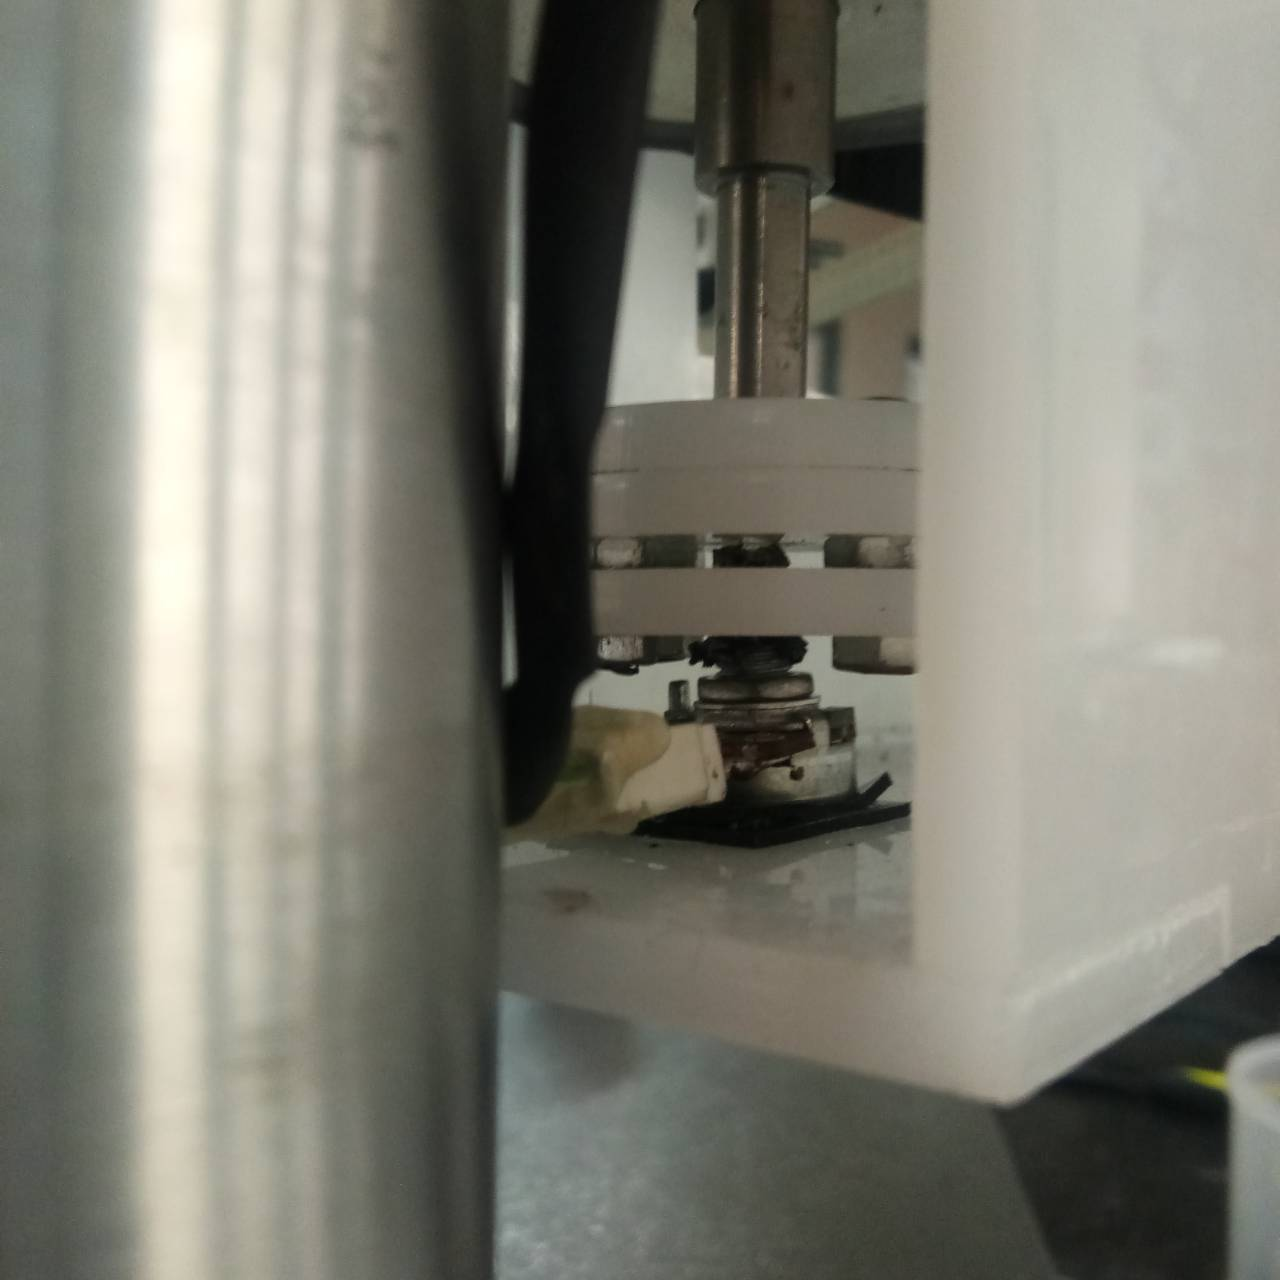
\includegraphics[width=5cm]{gambar/potsementara.jpg}
	\caption{Box Panel Robot SCARA}
	\label{pic.boxpanel}
\end{figure}

Pada \textit{arm manipulator robot} SCARA menggunakan penggerak berupa motor DC 12 Volt dengan \textit{gearbox} sehingga mampu mengangkat beban berat karena torsi pada motor bertambah besar. Motor DC dikontrol oleh \textit{Driver} Motor EMS 30A H-\textit{Bridge} melalui mikrokontroler Arduino Mega 2560. Tabel \ref{tbl.spesifikasimotordc} merupakan spesifikasi dari motor DC yang digunakan pada robot SCARA. 

	\begin{table}[H]
	\centering
	\caption{Spesifikasi Motor DC pada Robot SCARA}
	\label{tbl.spesifikasimotordc}
	\resizebox{15cm}{!}{%
		\begin{tabular}{|l|l|}
			\hline
			\rowcolor[HTML]{9B9B9B} 
			\multicolumn{1}{c|}{\cellcolor[HTML]{9B9B9B}Keterangan}		& \multicolumn{1}{c|}{\cellcolor[HTML]{9B9B9B}Nilai}			\\ \hline
			Moments of inertia of the main arm ($J_{1}$)    							& $0.0980kgm^{2}$ 				\\ \hline
			Moments of inertia of the fore arm ($J_{2}$)    							& $0.0115 kgm^{2}$ 				\\ \hline
			Masses of the main arm	($m_{1}$)											& $1.90kg$   					\\ \hline
			Masses of the fore arm  ($m_{2}$)     										& $0.93kg$   					\\ \hline
			Motor and equivalent inertias ($J_{m}$)      								& $3.3*10^{-6}kgm^{2}$ 			\\ \hline
			Back emf constants for main arm and fore arm motor ($K_{e1}=K_{e2}$)  		& $0.047Nm/A$   				\\ \hline
			Armature resistance for main arm and fore arm motor($R_{a1}=R_{a2}$)		& $3.5\Omega$  					\\ \hline
			Armatures inductances for main and fore arm motor  ($L_{a1}=L_{a2}$) 		& $1.3mH$ 						\\ \hline
		\end{tabular}%
	}
\end{table}
%%
Pada bagian \textit{gearbox} pada masing-masing motor DC terdapat \textit{potensiometer} sebagai sensor posisi. \textit{Potensiometer} ditempatkan pada bawah motor DC yang terhubung langsung. Setiap pergerakan dari motor DC, \textit{potensiometer} secara otomatis ikut bergerak dan kemudian mengirimkan nilai data analog ke Arduino Mega. Data yang berhasil diterima oleh Arduino Mega 2560 kemudian diolah dan mendapatkan hasil berupa besar sudut pada pergerakan \textit{joint} tersebut. Gambar \ref{pic.potensiometer} merupakan bentuk fisik dari motor DC serta pemasangan \textit{potensiometer}.
\begin{figure}[H]
	\centering
	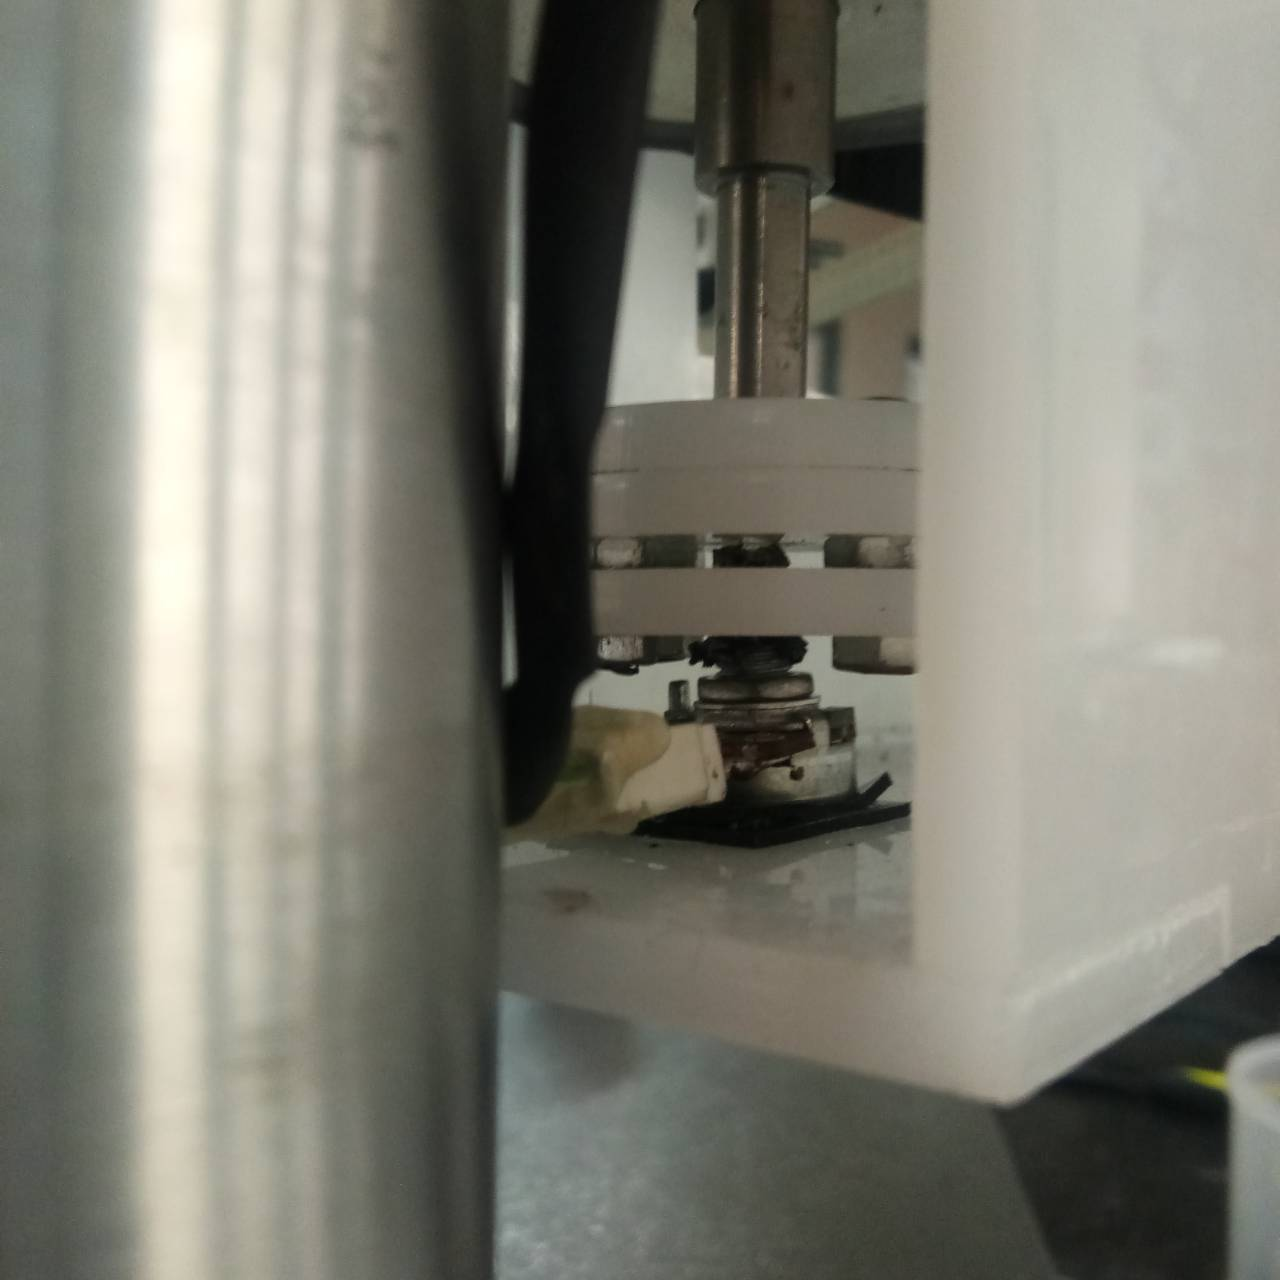
\includegraphics[width=5cm]{gambar/potsementara.jpg}
	\caption{Motor DC dengan \textit{Potensiometer}}
	\label{pic.potensiometer}
\end{figure}

Pada bagian \textit{end-effetor} menggunakan pergerakan translasi. Pergerakan translasi pada robot \textit{end-effector} merupakan gerak translasi pada sumbu Y. Pada robot SCARA pergerakan ini ada pada bagian \textit{end-effector} yang bergerak secara vertikal atau naik turun. Dengan pergerakan ini posisi \textit{end-effector} mengalami perubahan pada posisi tingginya. Pergerakan translasi juga terdapat pada bagian \textit{end-effector} yang menyebabkan sebuah \textit{gripper }\textit{ end-effector} dapat membuka dan menutup karena sebuah sistem mekanik yang telah ada di dalamnya. Selain dari pergerakan translasi, pergerakan pada end-effector juga terdapat rotasi. Pergerakan ini dilakukan oleh satu buah motor DC yang ditempatkan pada bagian \textit{shoulder} dengan dihubungkan melalui sebuauh \textit{belt}. Pengoperasian pada motor DC ini juga dilakukan oleh \textit{Driver} Motor EMS 30A H-\textit{Bridge}. Gambar \ref{pic.endeffectorfisik} merupakan bentuk fisik dari \textit{end-effector} pada robot SCARA yang digunakan. 
\begin{figure}[H]
	\centering
	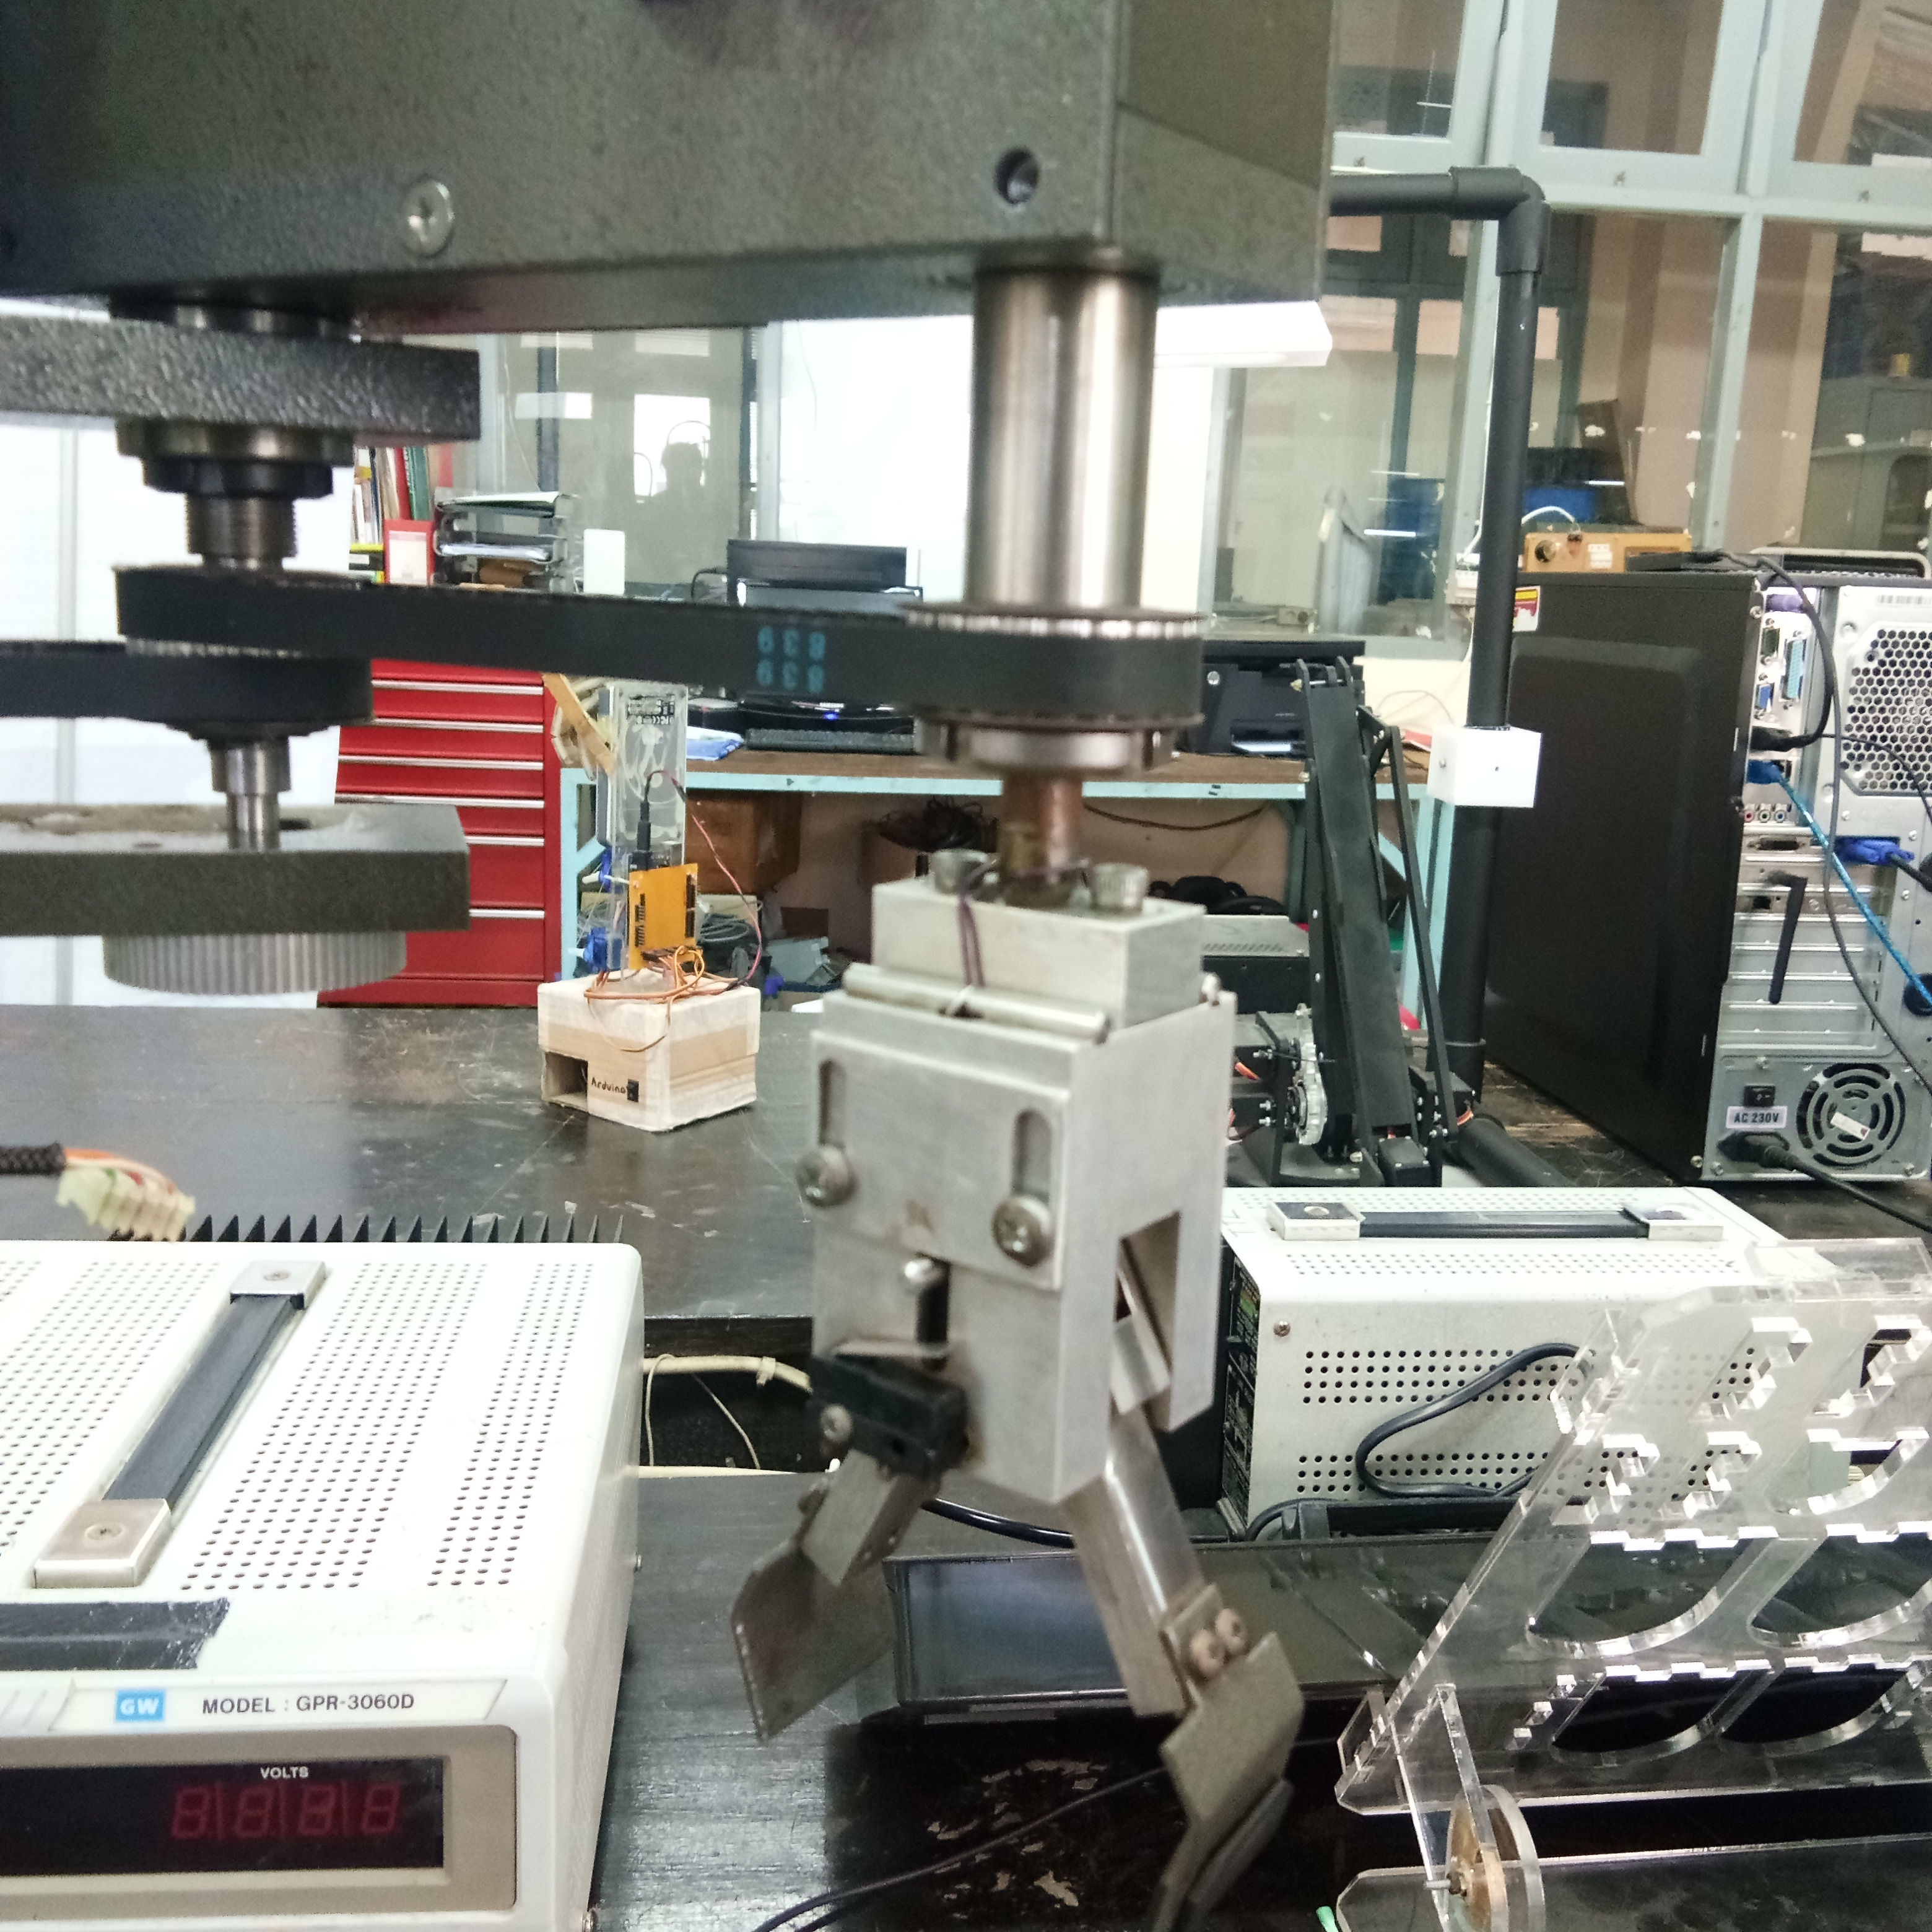
\includegraphics[width=5cm]{gambar/capitsementara.jpg}
	\caption{\textit{End-Effector} Robot SCARA}
	\label{pic.endeffectorfisik}
	
\end{figure}
Semua pergerakan pada \textit{end-effector} ditenagai oleh sebuah tekanan udara yang bersumber dari sebuah kompresor. Tekanan udara diaplikasikan pada sebuah \textit{pneumatic} dengan sistem kerja translasi yang dapat menyebabkan sebuah objek dapat bergerak pada sebuah garis lurus. Gambar \ref{pic.pneumatic} merupakan bentuk fisik dari \textit{pneumatic} yang digunakan pada robot SCARA. 
\begin{figure}[H]
	\centering
	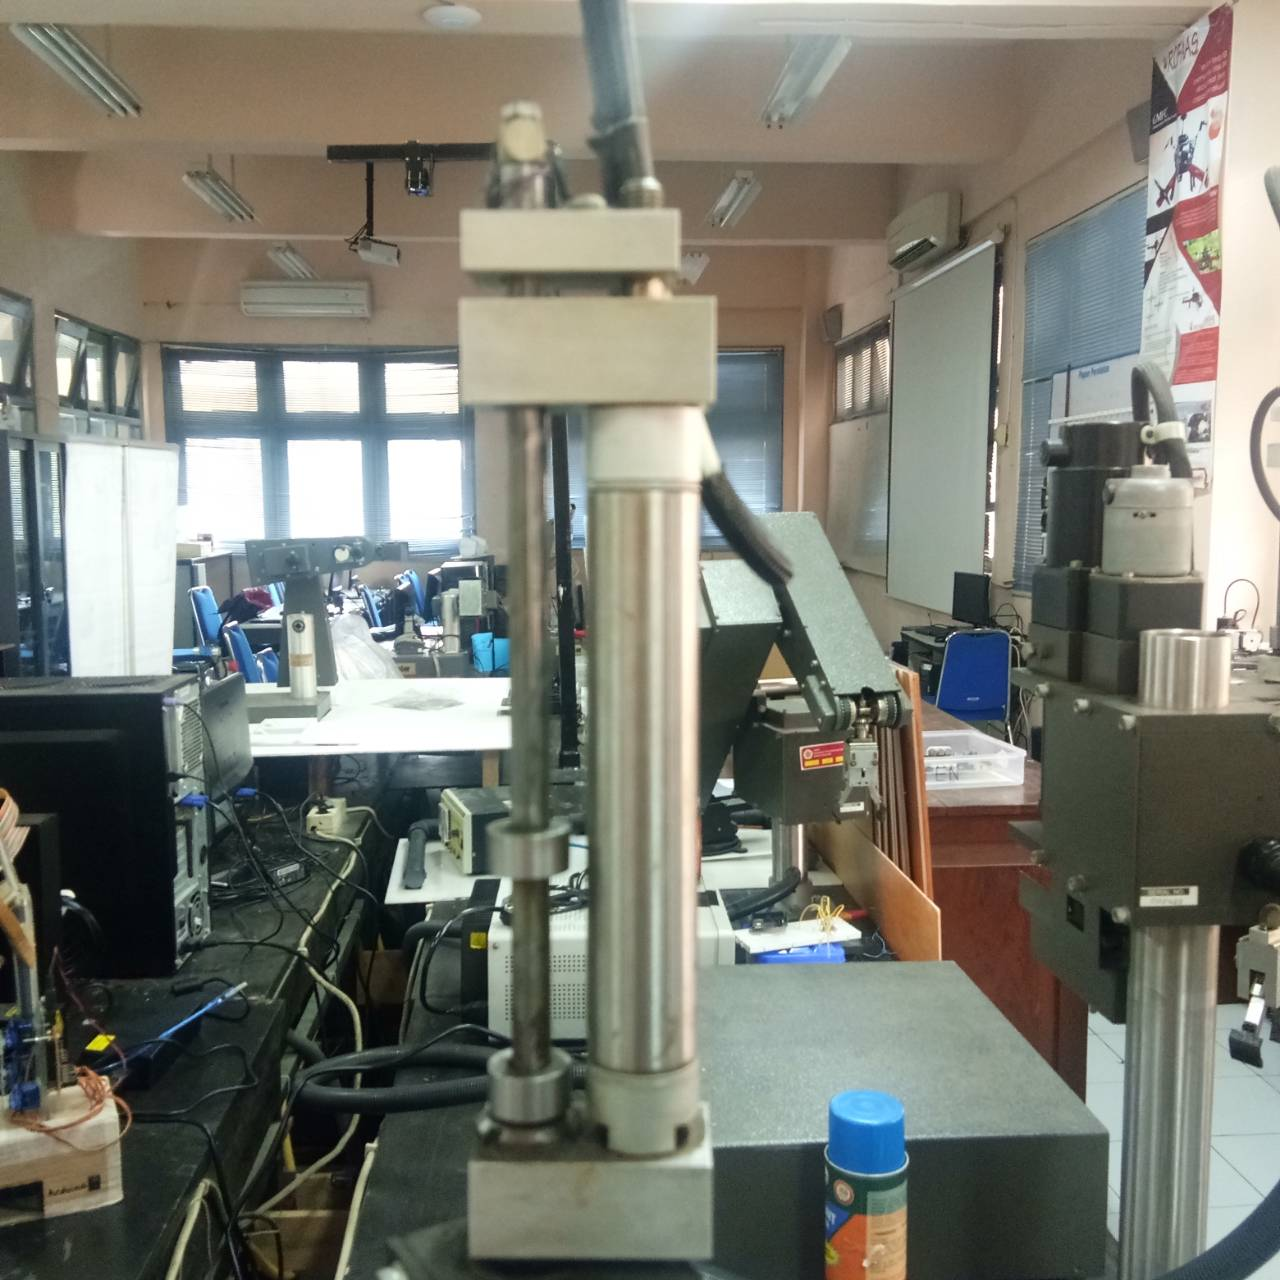
\includegraphics[height=6cm]{gambar/penuamticsementara.jpg}
	\caption{Bentuk Fisik \textit{Pneumatic}}
	\label{pic.pneumatic}
\end{figure}
Kompresor yang digunakan untuk menghasilkan sebuah tekanan udara merupakan sebuah kompresor listrik dengan kapasitas 8 bar. Kompresor ini dioperasikan menggunakan sumber tegangan AC 220 Volt. Ketika kapasitas udara sudah terpenuhi kompresor ini dapat digunakan tanpa menggunakan sumber tegangan tetapi hanya sebatas kapasitas udara yang disimpan. Gambar \ref{pic.kompresor} merupakan bentuk fisik dari kompresor yang digunakan.
\begin{figure}[H]
	\centering
	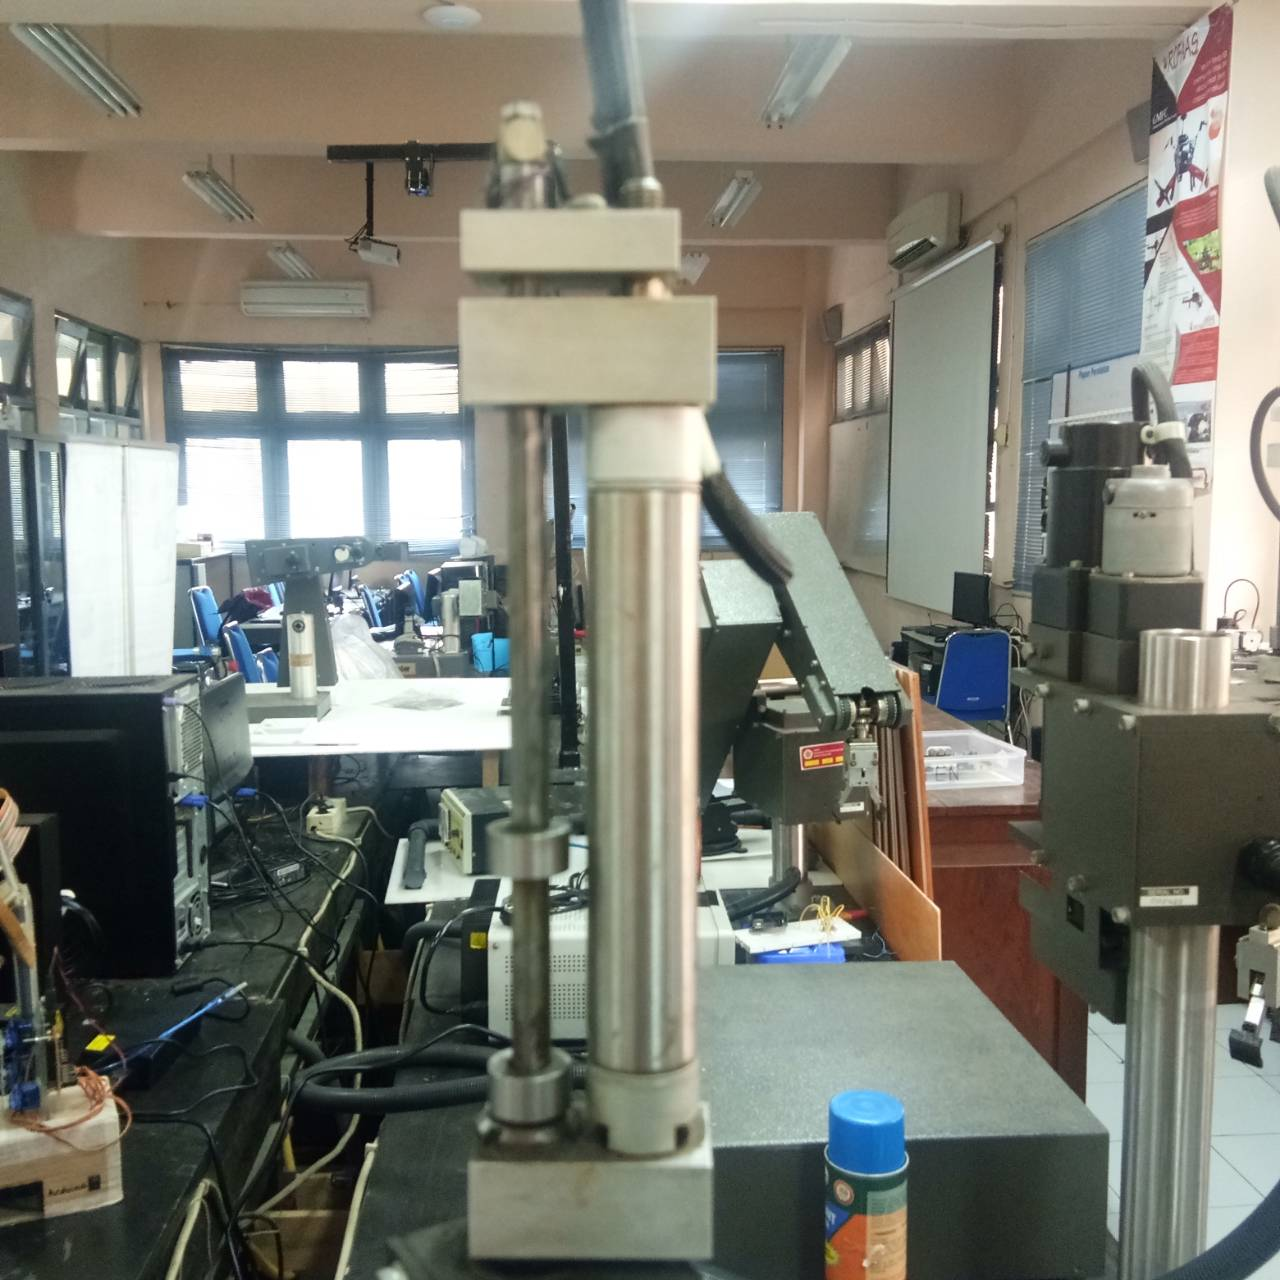
\includegraphics[height=6cm]{gambar/penuamticsementara.jpg}
	\caption{Bentuk Fisik Kompresor}
	\label{pic.kompresor}
\end{figure}

Rancangan robot secara keseluruhan ditampilan pada Gambar \ref{pic.scarasamping} yang merupakan rancangan tampak samping, Gambar \ref{pic.scaraatas} merupakan rancangan tampak atas dan Gambar \ref{pic.scaradimensi} merupakan rancangan dimensi robot. 
\begin{figure}[H]
	\centering
	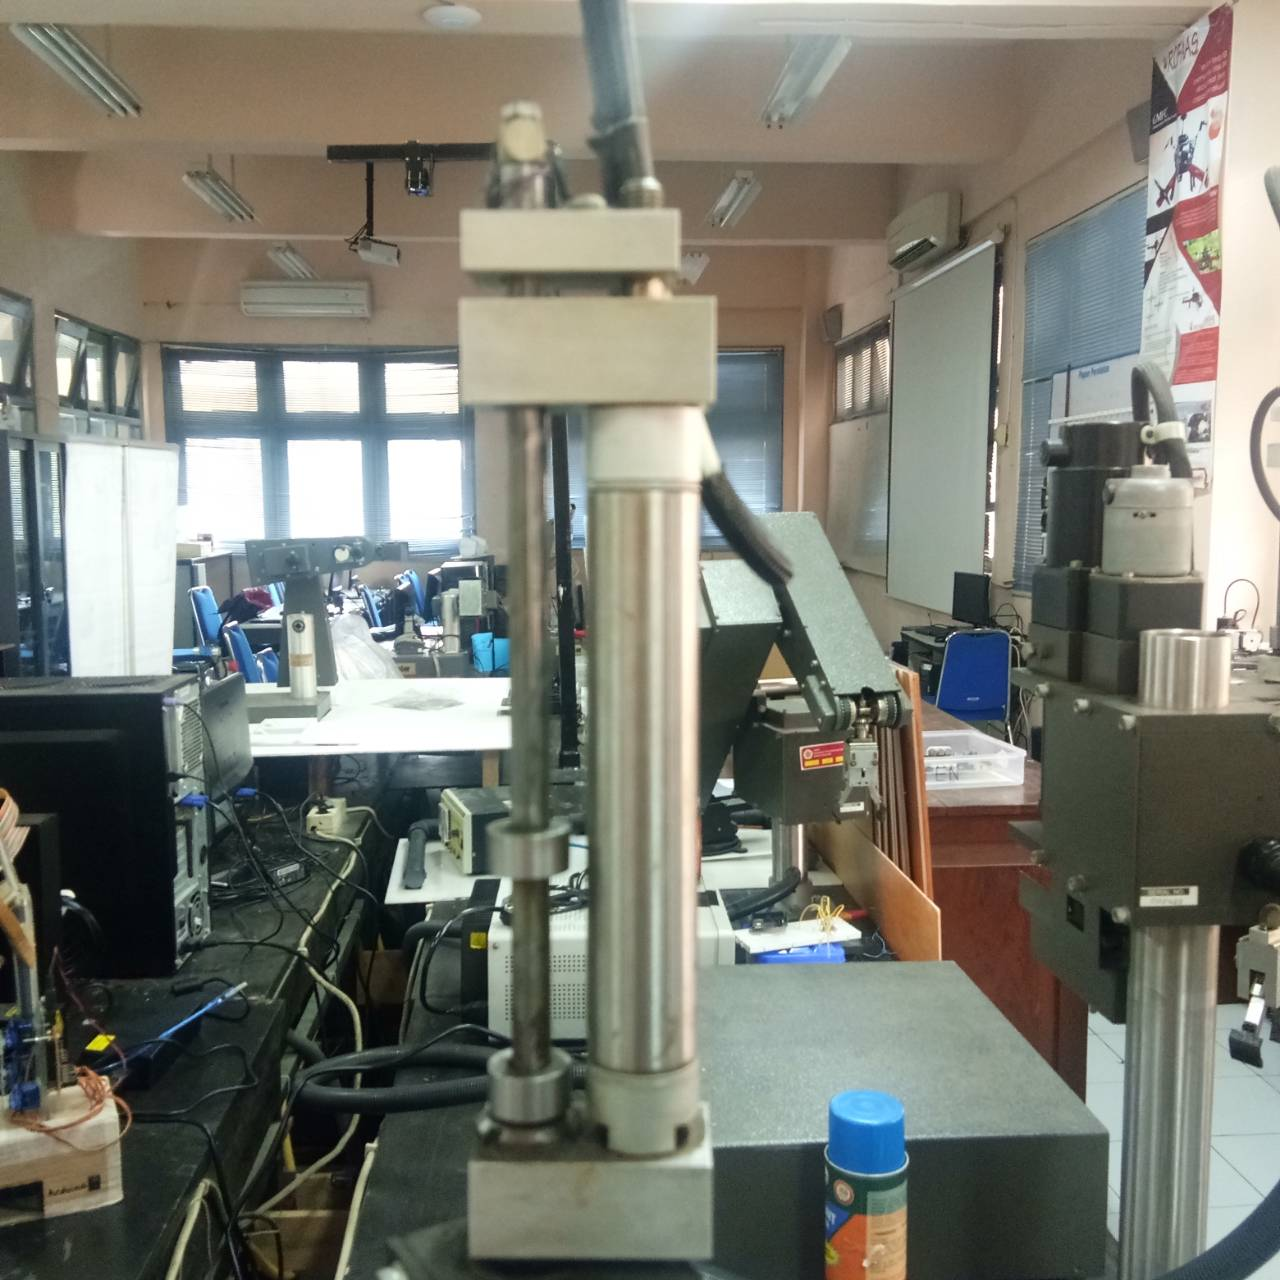
\includegraphics[height=6cm]{gambar/penuamticsementara.jpg}
	\caption{Rancangan Tampak Samping}
	\label{pic.scarasamping}
\end{figure}

\begin{figure}[H]
	\centering
	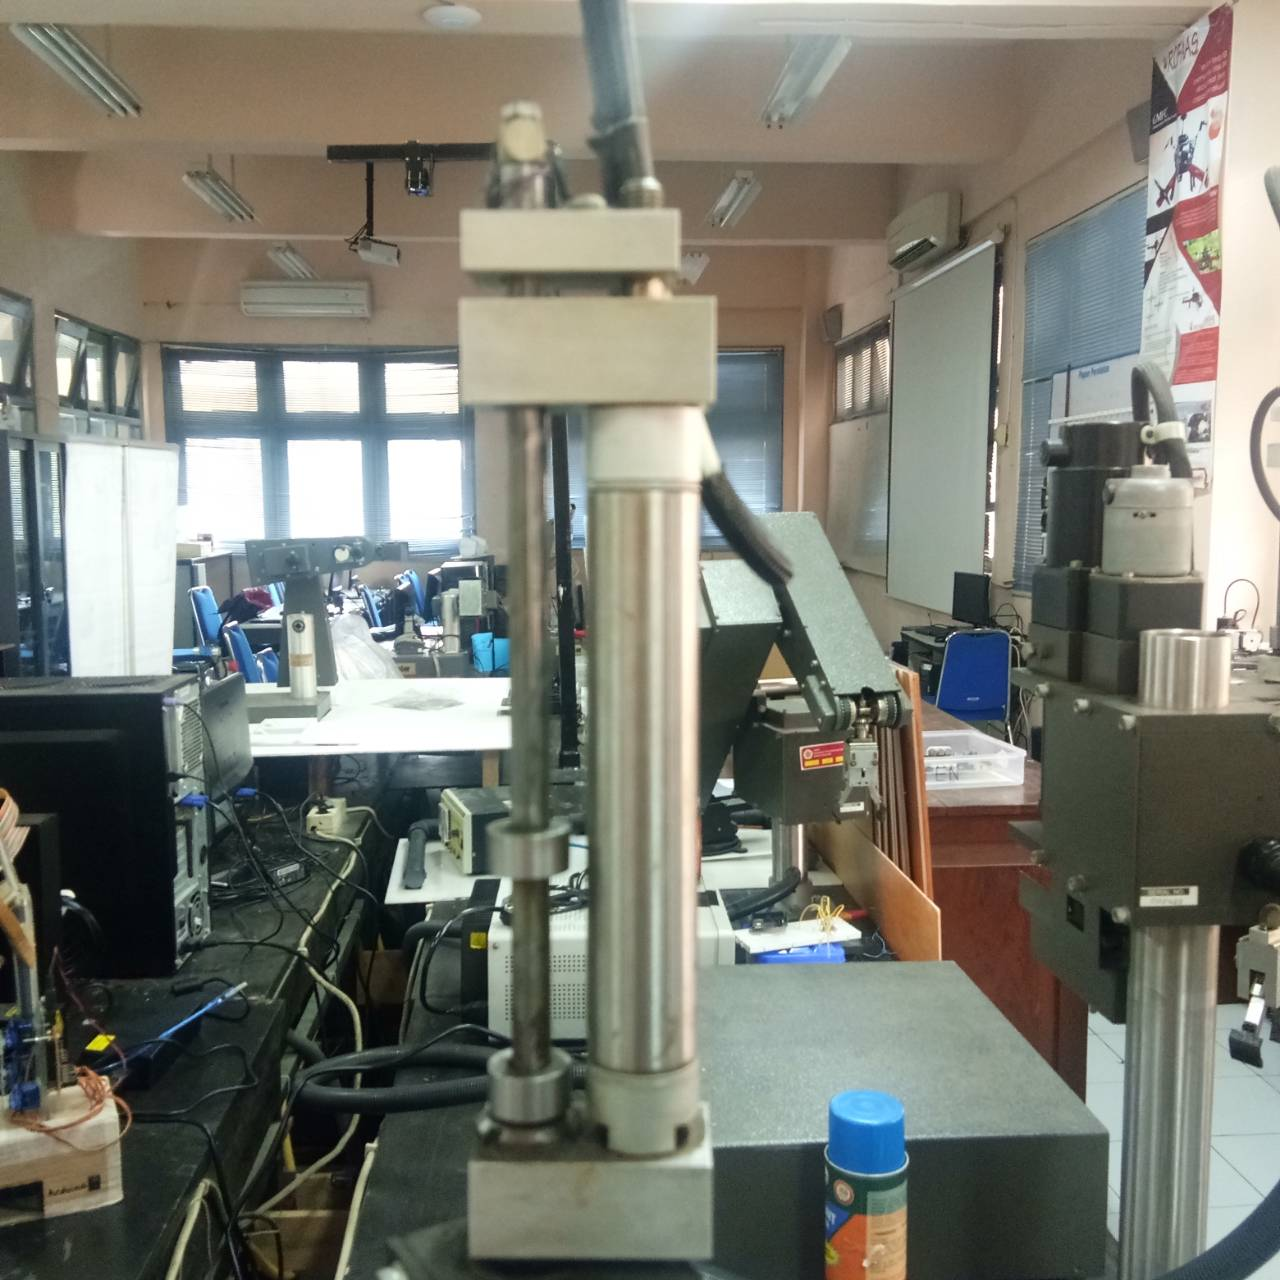
\includegraphics[height=6cm]{gambar/penuamticsementara.jpg}
	\caption{Rancangan Tampak Atas}
	\label{pic.scaraatas}
\end{figure}

\begin{figure}[H]
	\centering
	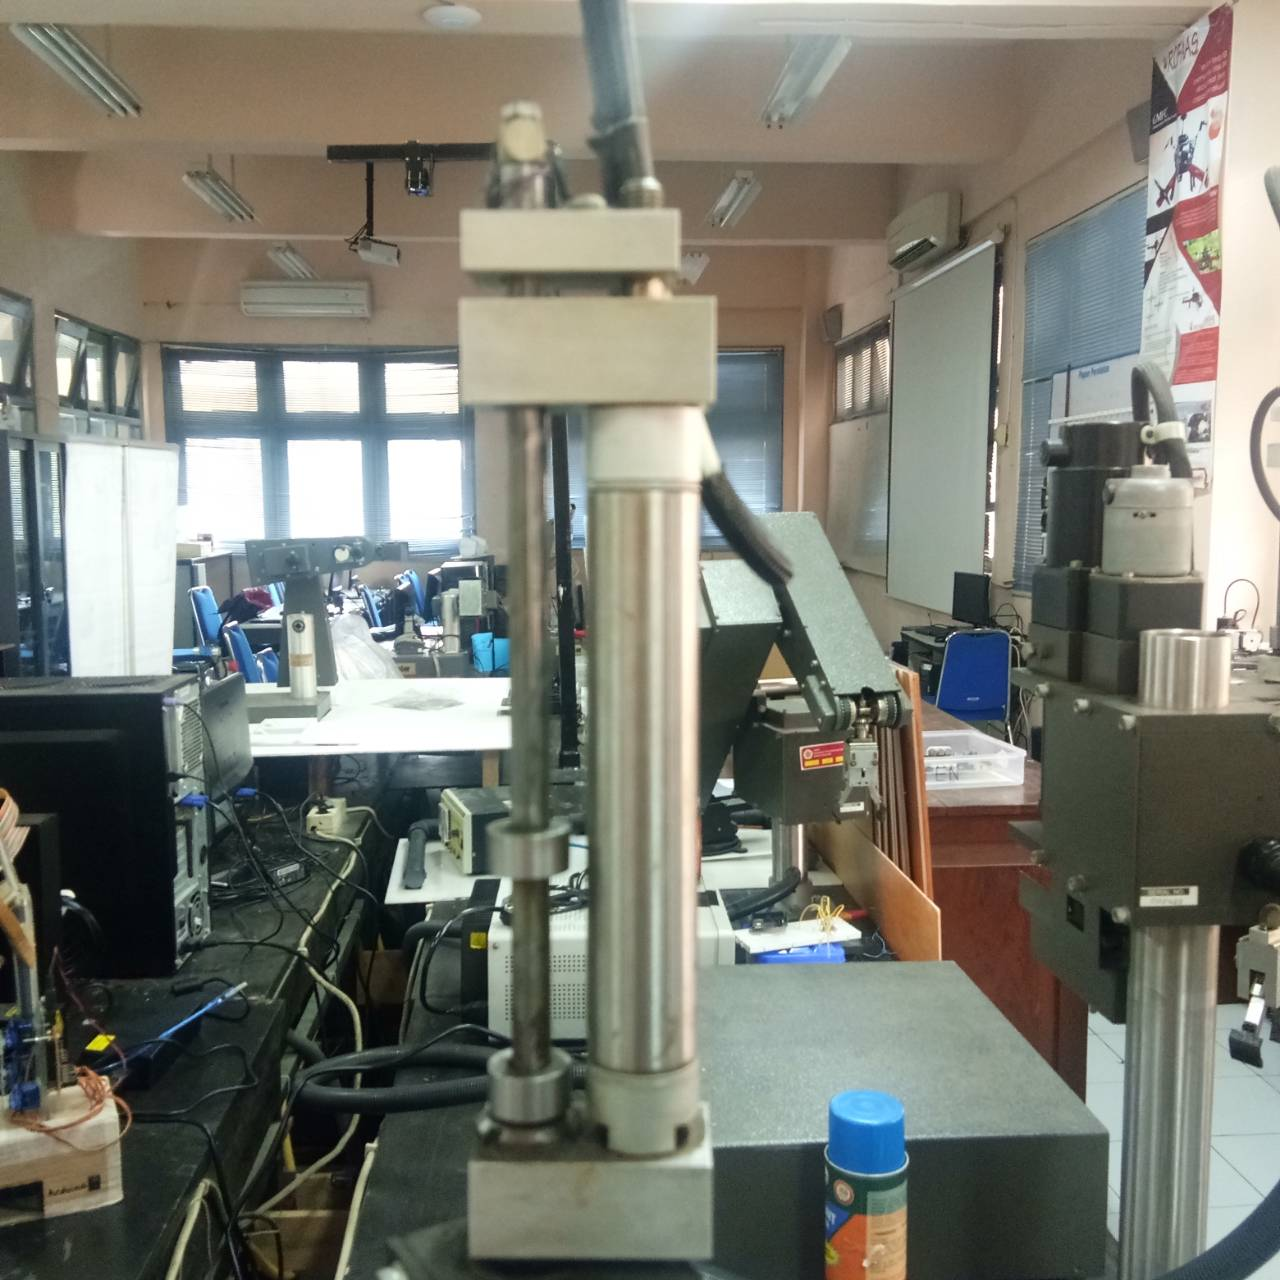
\includegraphics[height=6cm]{gambar/penuamticsementara.jpg}
	\caption{Dimensi Robot}
	\label{pic.scaradimensi}
\end{figure}

\subsection{Rangkaian Elektronika}
\subsubsection{Rangkaian Motor DC}
Rancangan kendali pada \textit{arm manipulator robot} SCARA ini menggunakan tiga buah motor DC dengan masing – masing dilengkapi dengan \textit{gearbox} untuk memperkuat torsi yang dihasilkan oleh motor DC. Pada  \textit{gearbox} masing – masing motor  DC diberikan sensor \textit{potensiometer} sebagai \textit{feedback} untuk memberikan posisi motor DC pada keseluruhan sistem. Motor DC diletakkan pada \textit{shoulder} untuk \textit{end-effector} satu buah yang dihubungkan melalui \textit{belt}, pada \textit{shoulder} satu buah, dan pada \textit{elbow} satu buah. Ketiga motor DC tersebut masing-masing menggunakan \textit{Driver} Motor EMS 30A H-\textit{Bridge} dalam sistem kerjanya. Pada masing – masing motor DC membutuhkan catu daya 12 Volt DC. Rangkaian \textit{driver} motor mendapat sumber tegangan DC 12V untuk disalurkan ke pada motor DC dan 5 Volt untuk kerja dari driver motor sendiri. 12 Volt didapat dari tegangan keluaran yang dihasilkan oleh regulator \textit{Buck} yang berseumber dari tegangan DC 24 Volt setelah dilakukan \textit{converter} AC to DC. Ragkaian utama \textit{Driver} Motor EMS 30A H-\textit{Bridge} ditunjukkan pada Gambar \ref{pic.drivermotor} dan pada Gambar \ref{pic.motordcdriver} merupakan rangkaian antara motor DC, driver motor, dan Arduino Mega.  
\begin{figure}[H]
	\centering
	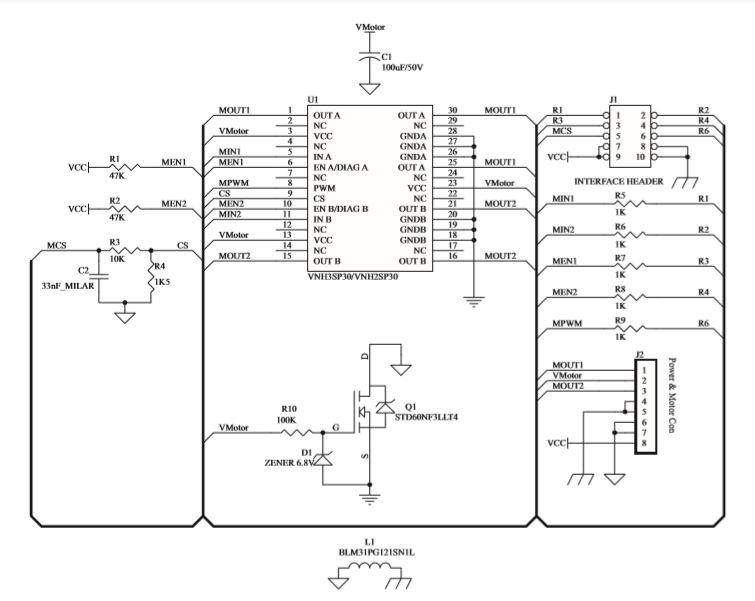
\includegraphics[width=10cm]{gambar/rangakaiandriver.jpg}
	\caption{Rangkaian Utama \textit{Driver} Motor EMS 30A H-\textit{Bridge}}
	\label{pic.drivermotor}
\end{figure}
\begin{figure}[H]
	\centering
	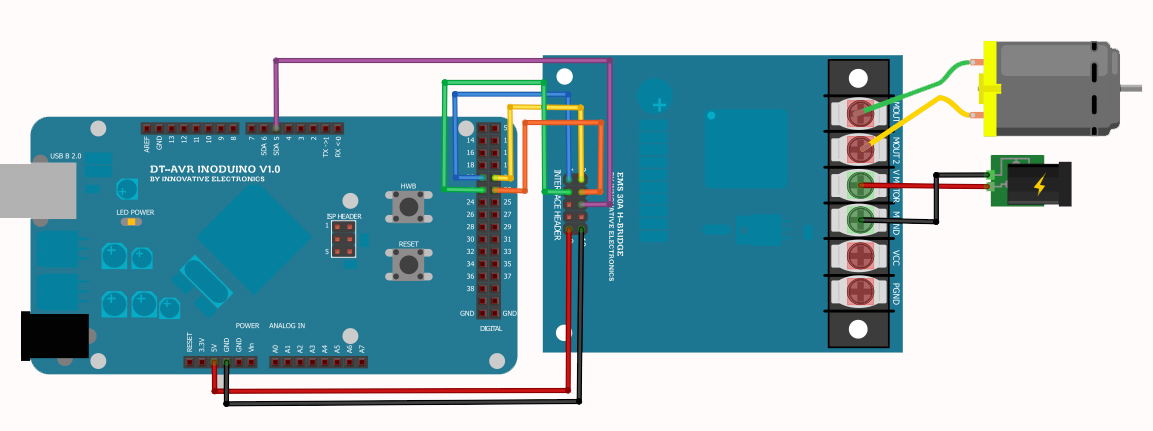
\includegraphics[width=10cm]{gambar/drivermotor.jpg}
	\caption{Rangkaian Arduino antara \textit{Driver} Motor dan Motor DC}
	\label{pic.motordcdriver}
\end{figure}
\subsubsection{Rangkaian \textit{Valve Pneumatic}}
\textit{End-Effector} menggunakan tekanan udara dalam melakukan pergerakannya. Tekanan udara ini dikontrol menggunakan sebuah\textit{valve relay}. \textit{Valve relay} yang digunakan dapat mengkontrol tekanan udara hingga delapan bar. \textit{Valve relay} dapat bekerja pada tegangan DC 24 Volt. Tegangan 24 Volt pada \textit{valve relay} didapat dari keluaran dari rangkaian AC-DC yang dilakukan oleh dioda \textit{bridge} dengan masukan awalnya adalah tegangan AC 24 Volt yang diberikan oleh sebuah tranformator. Dengan besaran tegangan 24 Volt maka sebuah arduino tidak dapat mengkontrolnya. Oleh karena itu, diberi sebuah rangkaian pembantu yang prinsipinya bekerja seperti saklar. Rangkaian tersebut diotaki oleh IC TIP31 yang nantinya akan menerima sinyal data digital dari Arduino Mega 2560 dan akan membuka jalur untuk tegangan 24 Volt. Gambar \ref{pic.fisikvalve} merupakan bentuk fisik dari \textit{valve relay} yang digunaakan dan Gambar \ref{pic.skematikvalve} merupakan rangkaian dari \textit{valve pneuamtic} dengan rangkaian TIP31.
\begin{figure}[H]
	\centering
	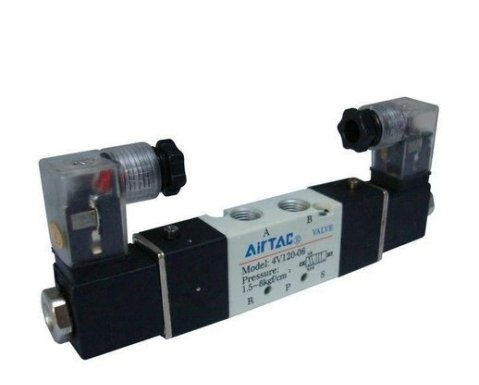
\includegraphics[width=5cm]{gambar/relay.jpg}
	\caption{Bentuk Fisik dari \textit{Valve Pneumatic}}
	\label{pic.fisikvalve}
\end{figure}
\begin{figure}[H]
	\centering
	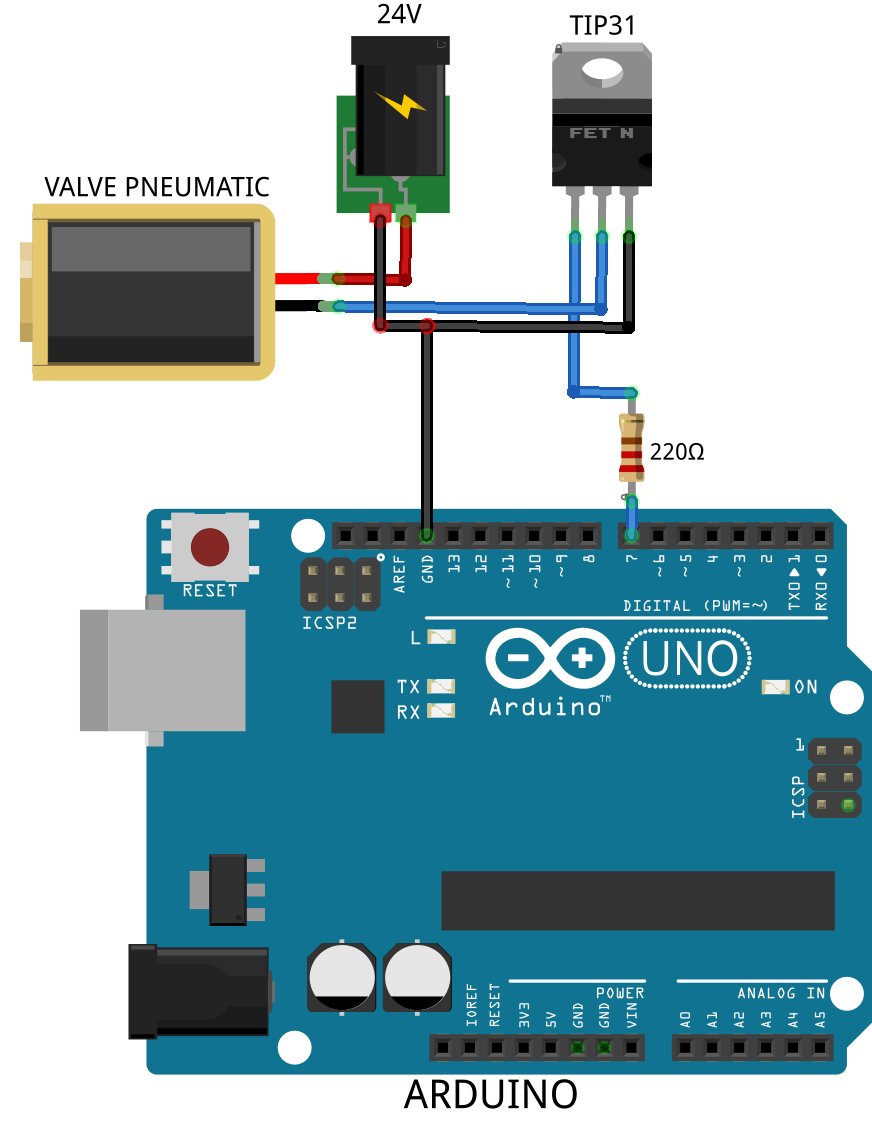
\includegraphics[width=5cm]{gambar/tip31.png}
	\caption{Rangkaian \textit{Valve Pneumatic} dengan Rangkaian TIP31}
	\label{pic.skematikvalve}
\end{figure}
\subsubsection{Rangkaian Minimum Sistem Arduino}
Arduino Mega 2560 digunakan sebagai mikrokontroler utama untuk mengendalikan seluruh sistem pada \textit{arm manipulator robot} SCARA. Arduino  2560 memiliki banyak pin keluaran dan masukan digital dan analog yang dapat digunakan sebagai pengendali fungsi – fungsi dari setiap komponen. Pin pada Arduino  2560 dapat mencukupi kebutuhan masukan dan keluaran untuk sistem kerja robot. Pin analog yang pada Arduino  digunakan untuk menerima \textit{feedback} masukkan dari potensio yang ada pada setiap motor robot. Beberapa pin digital pada Arduino Mega 2560 juga  memiliki fungsi lain yaitu sebagai pin \textit{Pulse With Modulation} (PWM) yang dapat digunakan sebagai keluaran analog sehingga dapat digunakan untuk mengatur nilai tegangan kaluaran dari Arduino  2560. Pin PWM yang cukup digunakan untuk kontrol kecepatan pada \textit{driver} motor. Selain itu pin PWM pada Arduino Mega 2560 digunakan untuk memberikan kontrol direksi pada \textit{driver} motor untuk memberikan masukan arah putar kanan ataupun putar kiri. Gambar \ref{pic.sisminarduino} merupakan rangkaian sistem minimum Arduino Mega 2560 pada robot SCARA ini. Tabel \ref{tbl.pinarduino} merupakan fungsi dari masing-masing pin yang ada pada Arduino Mega 2560.
\begin{figure}[H]
	\centering
	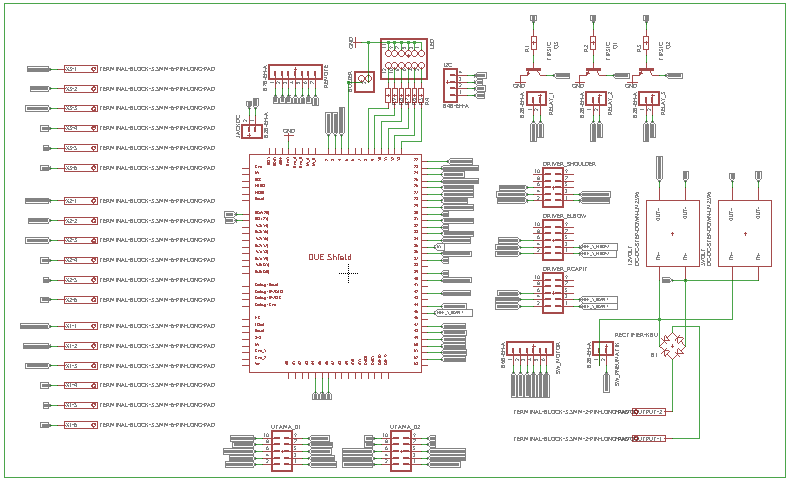
\includegraphics[width=15cm, height=10cm]{gambar/skematik1.png}
	\caption{Rangkaian Minimum Sistem Arduino}
	\label{pic.sisminarduino}
\end{figure}

\begin{table}[H]
		\centering
	\caption{Pin pada Arduino Mega 2560}
	\label{tbl.pinarduino}
	\begin{tabular}{|c|c|l|}
		\hline
		\rowcolor[HTML]{9B9B9B} 
		No & \begin{tabular}[c]{@{}c@{}}Pin Arduino\\   Mega 2560\end{tabular} & \multicolumn{1}{c|}{\cellcolor[HTML]{9B9B9B}Fungsi} \\ \hline
		1  & A1                                                                & Feedback potensiometer shoulder                     \\ \hline
		2  & A2                                                                & Feedback potensiometer elbow                        \\ \hline
		3  & A3                                                                & Feedback potensiometer end-effector                 \\ \hline
		4  & D16, D18                                                          & Kontrol aktif driver motor shoulder                 \\ \hline
		4  & D20, D22                                                          & Kontrol driver motor shoulder                       \\ \hline
		5  & D24, D26                                                          & Kontrol aktif driver motor elbow                    \\ \hline
		6  & D28. D30                                                          & Kontrol driver motor elbow                          \\ \hline
		7  & D32, D34                                                          & Kontrol aktif driver motor end-effector             \\ \hline
		8  & D36, D38                                                          & Kontrol driver motor end-effector                   \\ \hline
		9  & D4                                                                & Kontrol PWM driver motor shoulder                   \\ \hline
		10 & D5                                                                & Kontrol PWM driver motor elbow                      \\ \hline
		11 & D6                                                                & Kontrol PWM driver motor end-effector               \\ \hline
		12 & D7                                                                & Kontrol valve relay naik                            \\ \hline
		13 & D8                                                                & Kontrol valve relay turun                           \\ \hline
		14 & D9                                                                & Kontrol valve relay buka-tutup                      \\ \hline
		15 & D15                                                               & Kontrol LED Shoulder aktif high                     \\ \hline
		16 & D17                                                               & Kontrol LED elbow aktif high                        \\ \hline
		17 & D19                                                               & Kontrol LED end-effector naik aktif high            \\ \hline
		18 & D21                                                               & Kontrol LED end-effector turun aktif high           \\ \hline
		19 & D23                                                               & Kontrol LED end-effector buka-tutup aktif high      \\ \hline
		20 & D25                                                               & Buzzer aktif high                                   \\ \hline
	\end{tabular}
\end{table}

\subsubsection{Rangkaian Catu Daya}
Rangkaian catu daya merupakan hal yang sangat penting dalam sebuah sistem. Pada \textit{arm manipulator robot} SCARA terdapat tiga buah bilai tegangan \textit{supply} yang berbeda. Tegangan yang ditujukkan untuk Arduino Mega 2560 dan beberapa sensor membutuhkan tegangan 5 Volt, motor DC membutuhkan tegangan 12 Volt dan \textit{valve pneumatic} membutuhkan tegangan 24 Volt. Catu daya diawali dengan tegangan AC 220 Volt dari listrik PLN. Tegangan tersebut kemudian diturunkan menggunakan sebuah trafo 3A menjadi 24 Volt AC. Komponen yang digunakan dalam rangakaian merupakan komponen yang membutuhkan tegangan DC, maka tegangan 24 Volt AC diubah menjadi 24 Volt DC menggunakan rangkaian dioda \textit{bridge}. Tegangan 24 Volt DC diarahkan menuju dua buah regulator \textit{Buck} LM2596 yang masing-masing menghasilkan tegangan 12 Volt dan 5 Volt. Gambar \ref{pic.skematikcatu} merupakan rangkaian catu daya secara keseluruhan.
\begin{figure}[H]
	\centering
	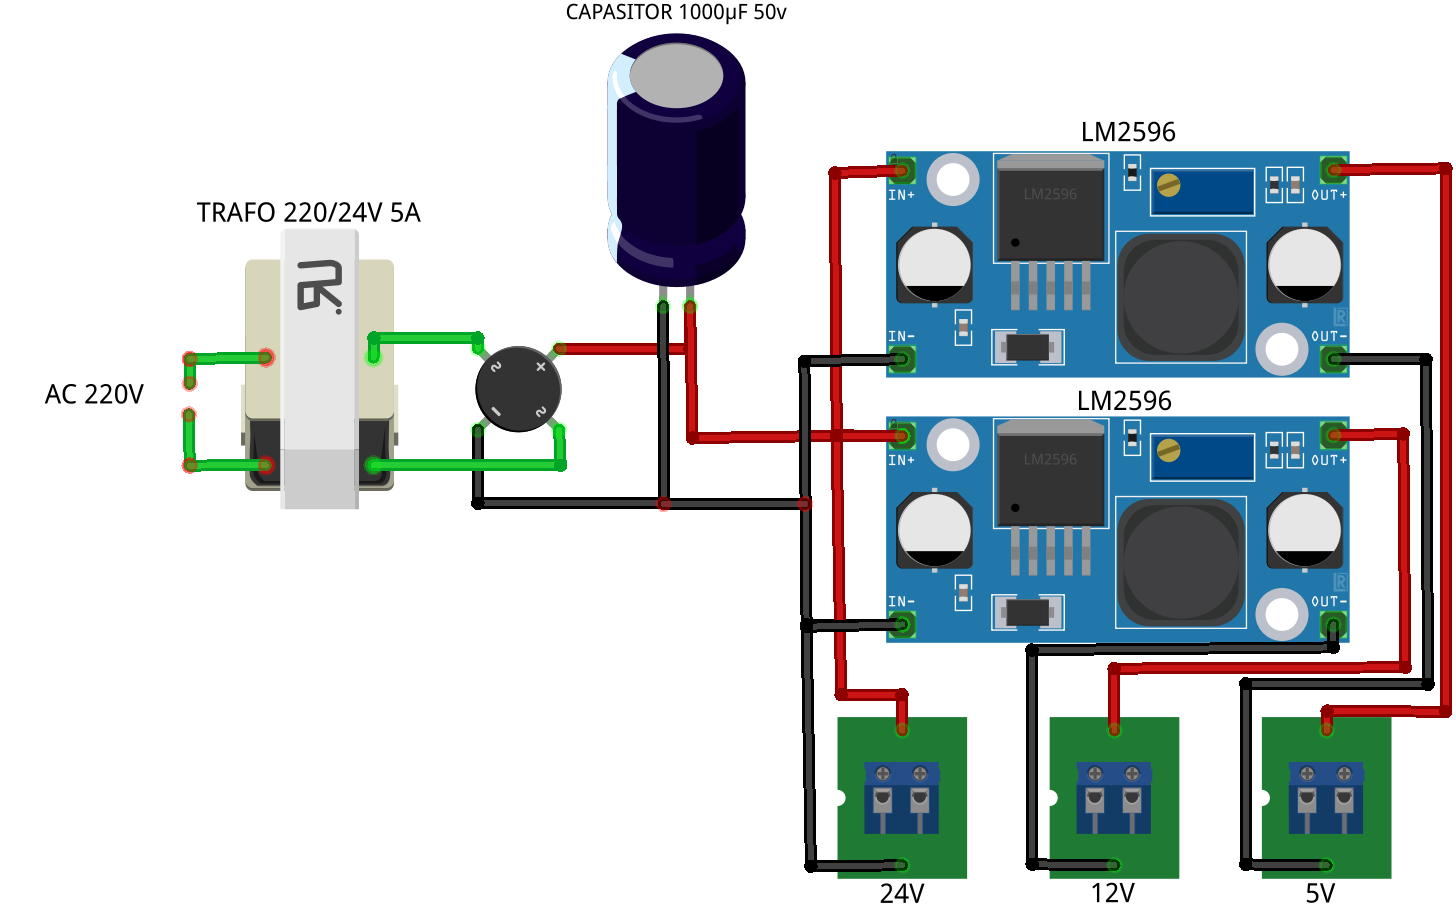
\includegraphics[width=8cm]{gambar/catudaya_bb.png}
	\caption{Rangkaian Catu Daya}
	\label{pic.skematikcatu}
\end{figure}
\section{Perancangan Perangkat Lunak}
Perangkat lunak yang digunakan merupakan \textit{software} Processing IDE. Processing IDE diprogram agar menghasilkan sebuah GUI yang cocok sesuai dengan fungsi robot SCARA. Di dalam GUI terdapat dua bagian yang diantaranaya merupakan bagian kontrol, dan bagian \textit{display}. Pada bagian kontrol pada GUI berfungsi untuk mengkontrol mulai dari pergerakan dan posisi dari robot SCARA. Sedangkan pada bagian penampil, GUI menampilkan nilai dari sudut, posisi, serta animasi terkait robot SCARA. Gambar \ref{pic.gui} merupakan tampilan dari GUI secara keseluruhan. Tabel \ref{tbl.gui} menyajikan setiap komponen yang ditampilan di dalam GUI processing IDE.
\begin{figure}[H]
	\centering
	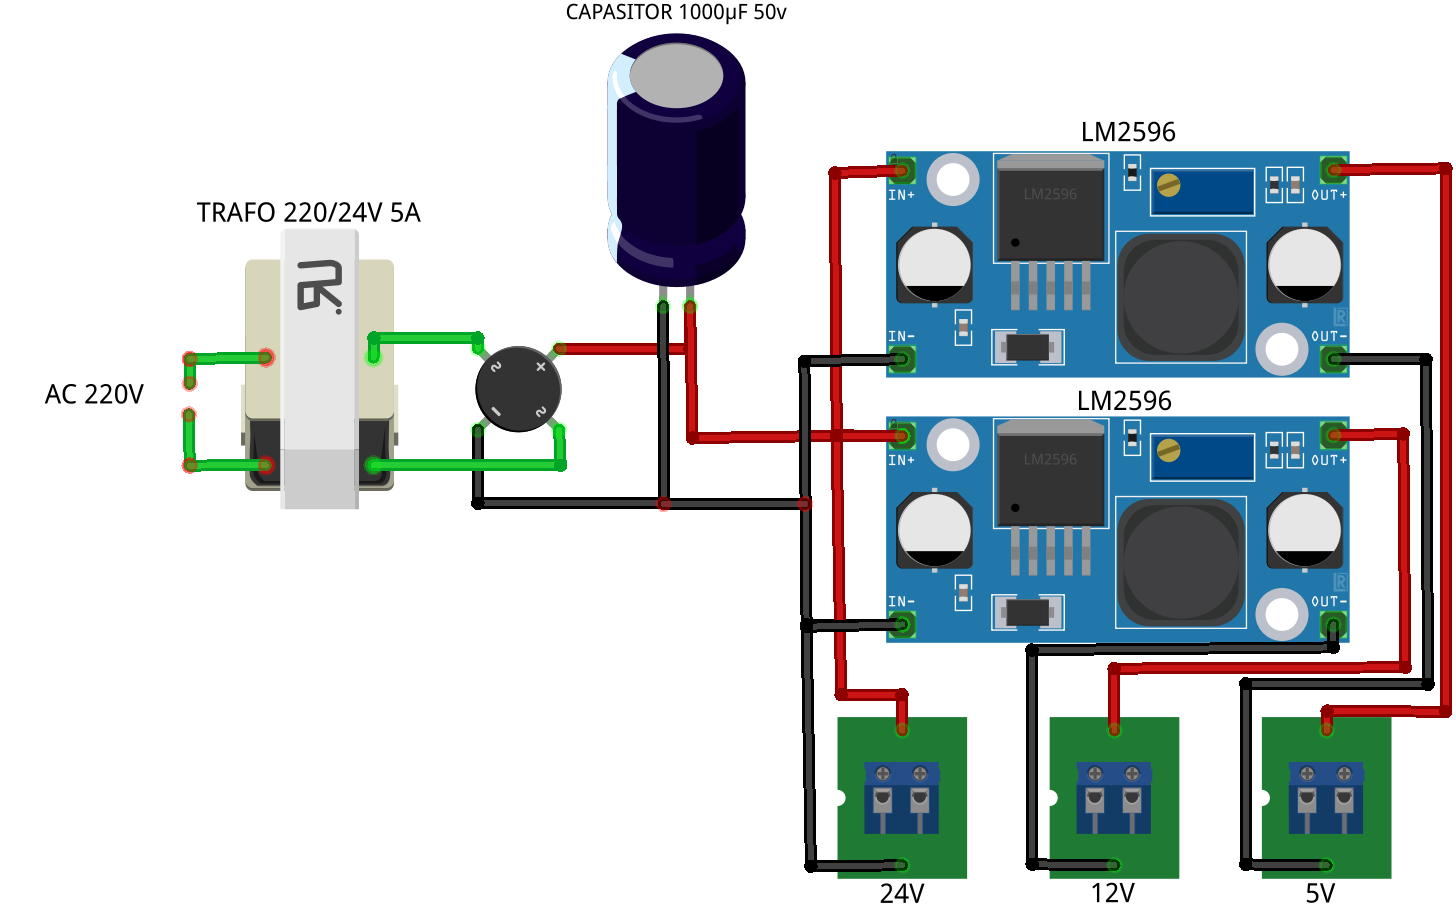
\includegraphics[width=10cm ]{gambar/catudaya_bb.png}
	\caption{Tampilan GUI Sistem Kinematika Robot SCARA}
	\label{pic.gui}
\end{figure}

\begin{table}[H]
	\centering
	\caption{Keterangan Tampilan pada GUI Robot SCARA}
	\label{tbl.gui}
	\begin{tabular}{|c|c|l|}
		\hline
		\rowcolor[HTML]{9B9B9B} 
		No & \begin{tabular}[c]{@{}c@{}}Pin Arduino\\   Mega 2560\end{tabular} & \multicolumn{1}{c|}{\cellcolor[HTML]{9B9B9B}Fungsi} \\ \hline
		1  & A1                                                                & Feedback potensiometer shoulder                     \\ \hline
		2  & A2                                                                & Feedback potensiometer elbow                        \\ \hline
		3  & A3                                                                & Feedback potensiometer end-effector                 \\ \hline
		4  & D16, D18                                                          & Kontrol aktif driver motor shoulder                 \\ \hline
		4  & D20, D22                                                          & Kontrol driver motor shoulder                       \\ \hline
	
	\end{tabular}
\end{table}


\subsection{ControlP5}
ControlP5 merupakan salah satu \textit{library} yang berguna dalam membuat sebuah GUI. Dalam \textit{library} yang disediakan terdapat banyak pilihan terkait kontrol sistem dengan berbagai jenis pilihan. Kontrol sistem yang disediakan tersedia dua pilihan yaitu untuk menkontrol dan untuk menampilkan sebuah data. Masing-masing kontrol sistem ini dapat digunakan dengan cara memanggilnya pada program yang ditulis.

Pada perancangan kineatika robot SCARA ini, menggunakan empat buah kontrol sistem. Empat kontrol sistem yang digunakan merupakan jenis kontrol sistem yang berguna untuk memberikan sebuah data yang dikirimkan pada Arduino Mega 2560. Kontrol sistem tersebut diantaranya:
\begin{enumerate}
	\item \textit{Slider Control} \\
	\textit{Slider Control} berupa tampilan kontrol GUI yang menggunakan sistem geser dalam memberikan data. Data memiliki batasan atas dan batas bawah yang dimasukkan dalam program. Keuntungan menggunakan kontrol sistem jenis ini adalah mudahnya dalam memberikan sebuah data yang berbeda.


	\item \textit{Textfield Control} \\
\textit{Textfield control} berupa tampila kontrol GUI yang menggunakan masukan nilai data sesuai apa yang dituliskan atau diketikkan secara langsung. Kelebihan menggunakan kontrol sistem jenis ini karena dapat memasukkan nilai data lebih spesifik secara langsung sesuai keiinginan.
	
	\item \textit{Bang Control} \\
\textit{Bang control}
Berbeda dengan kontrol sistem sebelumnya,\textit{ bang control }berupa kotak yang bekerja pada saat mulai ditekan. Saat \textit{bang} mulai ditekan data akan dikirimkan sesuai dengan nilai yang sudah dimasukan kedalam program. 
	

	\item \textit{Toggle Control} \\
\textit{Toggle control}
\textit{Toggle control} memiliki sistem kontrol seperti saklar on-off. Pada saat ditekan maka \textit{toggle control} menyimpan data berupa kondisi pertama dan berubah saat ditekan kembali. 

\end{enumerate}
\subsection{\textit{Shape}}
\textit{Shape} pada GUI berfungsi sebagai penampil animasi tiga dimensi dari robot SCARA. Robot SCARA dapat ditampilkan dalam berbagai ukuran, letak dan juga dapat bergerak sesuai dengan data yang diberikan. Pergerakan dari robot SCARA merupakan implementasi dari wujud aslinya dengan pergerakan yang sama.

Dalam pengoperasianya, desain dari robot SCARA yang ditampilkan harus dimasukkan ke dalam folder yang sama dengan program processing IDE. File yang dapat ditampilkan merupakan file dengan jenis obj. yang berarti file objek. Pada program robot SCARA file dari dimensi tiga dari robot SCARA memiliki tiga buah file dimana ketiganya adalah \textit{base, shoulder}, dan \textit{elbow}. 

\section{Sistem Kinematika}
Persamaan kinematika terbagi dua, yaitu kinematika maju dan kinematika balik. Kinematika maju digunakan untuk menentukan posisi dan orientasi \textit{end-effector} apabila variabel sudut \textit{joint}-nya telah diketahui. Kinematika balik digunakan untuk mencari \textit{joint} robot dalam menentukan posisi dan orientasi dari \textit{end-effector.}
\subsection{Prinsip Kerja Kinematika Maju}
Metode Denavit-Hartenberg merupakan metode yang menggabungkan proses perhitungan rotasi dan translasi menjadi sebuah matriks yang menyertakan nilai-nilai sudut putar dan jarak sendi dari sebuah lengan robot. Dalam beberapa aplikasi, metode Denavit-Hartenberg umumnya digunakan dalam perhitungan \textit{Forward Kinematics}. Dalam penelitian ini dirancang aplikasi yang menggunakan metode Denavit-Hartenberg untuk menghitung sudut-sudut tiap sendi pada \textit{Invers Kinematics} untuk menggerakan sebuah lengan robot. Matrik Denavit-Hartenberg yang berisi perhitungan rotasi dan translasi digunakan untuk mendapatkan nilai nilai sudut untuk menggerakkan tiap motor sendi. Empat Aturan Frame Denavit-Hartenberg yaitu Sumbu Z harus menjadi sumbu rotasi atau translasi dari sebuah joint. Sumbu X harus tegak lurus dari sumbu Z frame sebelumnya. Sumbu X harus memotong atau menyilang dari sumbu Z frame sebelumnya. Sumbu Y harus digambarkan sesuai dengan aturan tangan kanan setelah sumbu X   dan sumbu Z setiap frame digambarkan.
\subsection{Prinsip Kerja Kinematika Balik}
Kinematika balik adalah perhitungan untuk mencari variabel sudut (\textit{joint}) robot dalam menentukan posisi dan orientasi dari \textit{end-effector}. Dalam menentukan koordinat \textit{end-effector}, kinematika balik harus disesuaikan dengan batas area kerja \textit{(workspace)} dari jangkauan robot. Penyelesaian kinematika balik ini dapat diselesaikan dengan menggunakan persamaan kinematika balik yang di dalamnya menggunakan hukum \textit{phytagoras} dan aturan \textit{cosinus}. 
Secara garis besar metode \textit{inverse kinematic} akan mencari nilai-nilai parameter yang harus diberikan kepada setiap aktuator untuk mencapai tujuan akhir. Untuk mendapatkan nilai-nilai parameter tersebut, robot harus mengetahui terlebih dahulu manipulator yang dimilikinya, baik ukuran maupun jumlah aktuator serta derajat kebebasan yang ada. Kemudian, robot harus ditanamkan rumus-rumus yang didapat dari berbagai model perhitungan, baik dari segi analisa grafik langsung maupun menggunakan metode-metode dari berbagai penelitian. 

Analisis persamaan kinematik dapat diselesaikan dengan cara yang paling dasar yaitu menggunakan trigonometri dengan bantuan grafik. Pada penelitian ini karena menggunakan sebuah GUI yang didalamnya terdapat animasi dari bentuk fisik robot SCARA maka koordinat didapat dari Processing IDE. Robot SCARA yang terdapat di dalam Processing IDE menggunakan skala tertentu agar tetap sesuai dari dimensi aslinya. Penyelesaian kinematika dalam robot SCARA cukup diselesaiakan menggunakan satu sisi, yaitu sisi atas (\textit{top view}) dari struktur robot lengan. Pada sisi atas derajat sudut \textit{joint} \textit{shoulder}, dan sudut \textit{joint elbow} dapat ditemukan. Gambar \ref{pic.perskinematikabalik} merupakan gambaran untuk mendapatkan sebuah persamaan yang akan menghasilkan nilai sudut pada setiap \textit{joint.}
\begin{figure}[H]
	\centering
	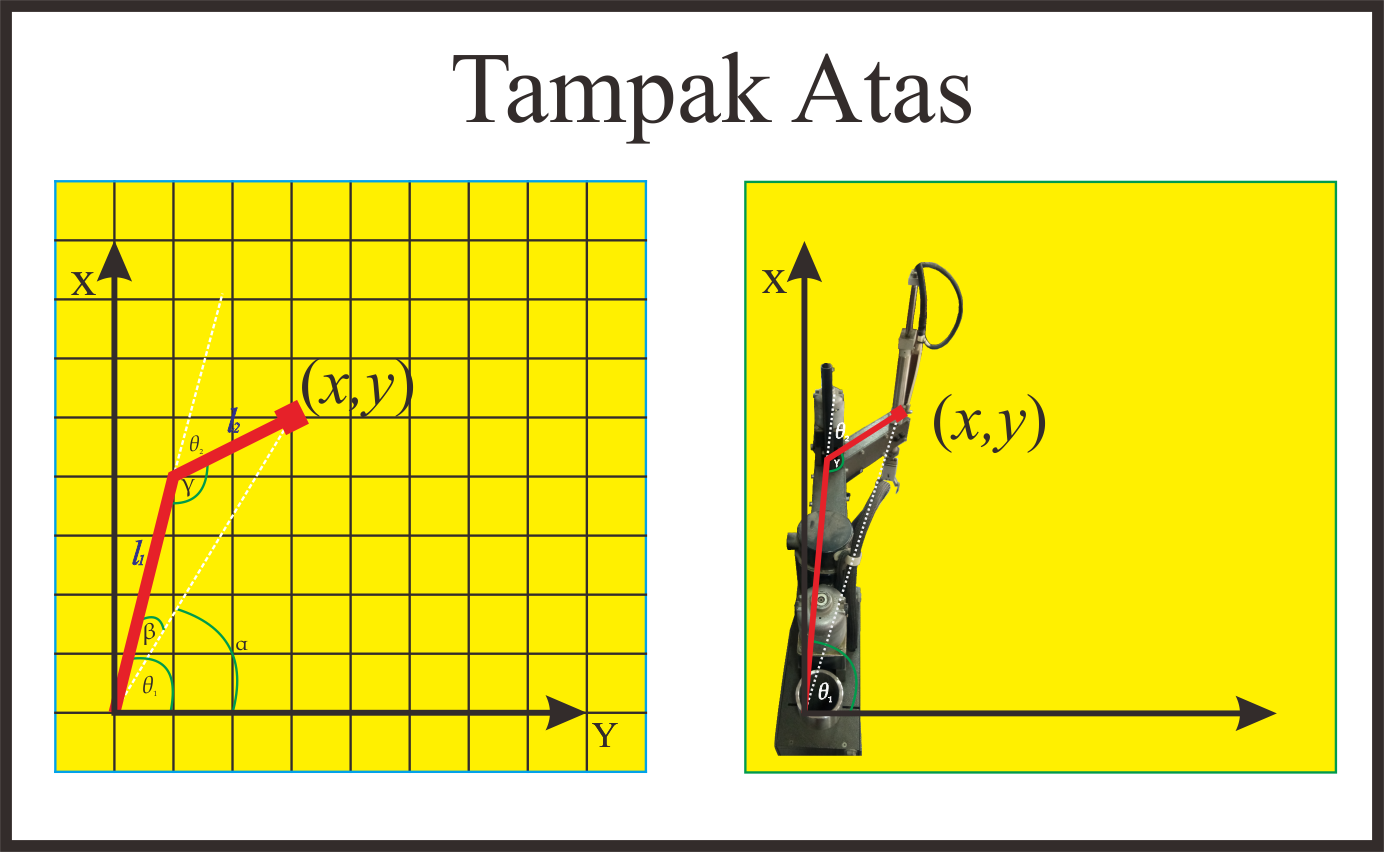
\includegraphics[width=12cm]{gambar/scara_atas.png}
	\caption{Trigonometeri Sisi Atas}
	\label{pic.perskinematikabalik}
\end{figure}
 
 
Pada robot SCARA, sudut dari \textit{joint} yang dicari merupakan \textit{joint} dari \textit{shoulder} dan juga \textit{elbow.} Kedua \textit{joint} tersebut dapat ditemukan dengan melalui persamaan \textit{pythagoras} dan juga hukum \textit{cosinus}. Pada Gambar \ref{pic.perskinematikabalik} terlihat bahwa sudut \textit{shoulder} merupakan besar sudut diantara lengan \textit{shoulder} dan juga sumbu $x$ dan sudut \textit{elbow} merupakan besar sudut antara lengan \textit{elbow} dengan garis bantu dari lengan \textit{shoulder}. Keduanya dapat ditentukan besar nilainya melalui beberapa pesamaan dari \textit{cosinus} dan juga hukum \textit{pyhtagoras}. $l_{1}$ merupakan panjang lengan \textit{shoulder} dan $l_{2}$ merupakan panjang lengan dari \textit{elbow}. Serta $\theta_{1}$ merupakan sudut dari \textit{shoulder} dan $\theta_{2}$ merupakan sudut dari \textit{elbow}.  

\begin{enumerate}
	\item Dengan menggunakan hukum \textit{cosinus}, didapatkan sebuah persamaan \ref{cosinus1}
	\begin{equation}
	(x^2+y^2)=l_{1}^2+l_{1}^2-2l_{2}l_{2}cos(180-\theta_{2})
	\label{cosinus1}
	\end{equation}
	\item Pada persamaan \ref{cosinus2} terdapat $\cos$ yang dapat diubah sesuai dengan prinsip dari hukum \textit{cosinus} menjadi seperti pada persamaan \ref{cosinus2}
	\begin{equation}
	(x^2+y^2)=l_{1}^2l_{2}^2+2l_{2}l_{2}cos(\theta_{2})
	\label{cosinus2}
	\end{equation}
	\item Inti persamaan akan mencari sebuah nilai dari $\theta_{2}$, maka untuk memmudahkannya maka persamaan menjadi seperti pada persamaan \ref{cosinus3}
	\begin{equation}
	cos(\theta_{2})=\frac{x^2+y^2-l_{1}^2-l_{2}^2}{2_{1}l_{2}}
	\label{cosinus3}
	\end{equation}
	\item Nilai dari $\theta_{2}$ dapat dengan mudah diketahui dengan melanjutkan seperti pada persamaan \ref{cosinus4}
	\begin{equation}
	\theta_{2}=arccos(\frac{x^2+y^2-l_{1}^2-l_{2}^2}{2_{1}l_{2}})
		\label{cosinus4}
	\end{equation}
	Dengan persamaan \ref{cosinus4} maka nilai dari $\theta_{2}$ atau sudut dari \textit{elbow} dapat diketahui dengan cara memasukkan nilai posisi $x$, posisi $y$ serta panjang dari \textit{shoulder} dan \textit{elbow} ke dalam persamaan. Nilai posisi $x$ dan posisi $y$ merupakan posisi akhir dari \textit{end-effector}. 
	\item Dalam menentukan sudut lainnya yaitu sudut \textit{shoulder} yang ditandai dengan simbol $\theta_{1}$ menggunakan persamaan \textit{cosinus} yang dituliskan pada persamaan \ref{cosinus5}
	\begin{equation}
	\frac{sin(\beta)}{l_{2}} = \frac{sin(\gamma)}{\sqrt{x^2+y^2}} ; \alpha=\arctan(\frac{y}{x})
	\label{cosinus5}
	\end{equation}
	\item Pada persamaan \ref{cosinus5} beberapa dapat diubah sesuai dengan hukum \textit{cosinus} $\sin(\gamma)=\sin(180-\theta_{2})=\sin(\theta_{2})$ dengan mengubah $\sin(\gamma)$ menjadi $\sin(\theta_{2})$ maka akan persamaan menjadi seperi yang ditunjukkan pada persamaan \ref{cosinus6}
	\begin{equation}
	\beta=\arcsin(\frac{l_{2}\sin(\theta_{2})}{\sqrt{x^2+y^2}})
	\label{cosinus6}
	\end{equation}
	\item Jika dilihat pada gambar \ref{pic.perskinematikabalik} maka besar dari sudut \textit{shoulder} yang ditandakan dengan $\theta_{1}$ yang artinya $\theta_{1}=\beta+\alpha$ maka dapat diselesaikan dengan persamaan \ref{cosinus7}
	\begin{equation}
	\theta_{1}=\arcsin(\frac{l_{2}\sin(\theta_{2})}{\sqrt{x^2+y^2}}+\arctan(\frac{y}{x})
	\label{cosinus7}
	\end{equation}
	\item  Dengan penyelesaian seperti pada persamaan \ref{cosinus7} besar sudut dari \textit{shoulder} dapat diketahui dengan memasukkan nilai panjang \textit{elbow}, sudut \textit{elbow} dan juga posisi dari \textit{end-effector}.
\end{enumerate}

Dalam penelitian kinematika robot SCARA ini, segala perhitungan kinematika dilakukan di dalam program processing IDE. Di dalam processing IDE terdapat animasi dari bentuk asli robot SCARA dengan dimensi yang sama hanya saja ditampilkan dalam bentuk berskala. Pada posisi \textit{end-effector} didapat posisi $x$ dan $y$ yang diprogram pada dalam processing IDE. Dua buah data sudut yang didapat pada perhitungan merupakan sudut \textit{shoulder} dan \textit{elbow} kemudian dikirimkan kepada Arduino Mega 2560 untuk diprores dan diimplemintasikan secara langsung pada robot lengan.

\section{Perancangan Sistem Keseluruhan}
Rancangan sistem keseluruhan merupakan gabungan dari perancangan perangkat keras dan perangkat lunak yang diintegrsikan sesuai dengan diagram blok sistem. Gambar \ref{pic.sistemkeseluruhan} adalah gambaran tentang perancangan sistem secara keseluruhan. Tabel \ref{tbl.sistemkeseluruhan}  menunjukkan keterangan setiap komponen yang ada di dalam sistem keseluruhan \textit{arm manipulator} robot SCARA. 
\begin{figure}[H]
	\centering
	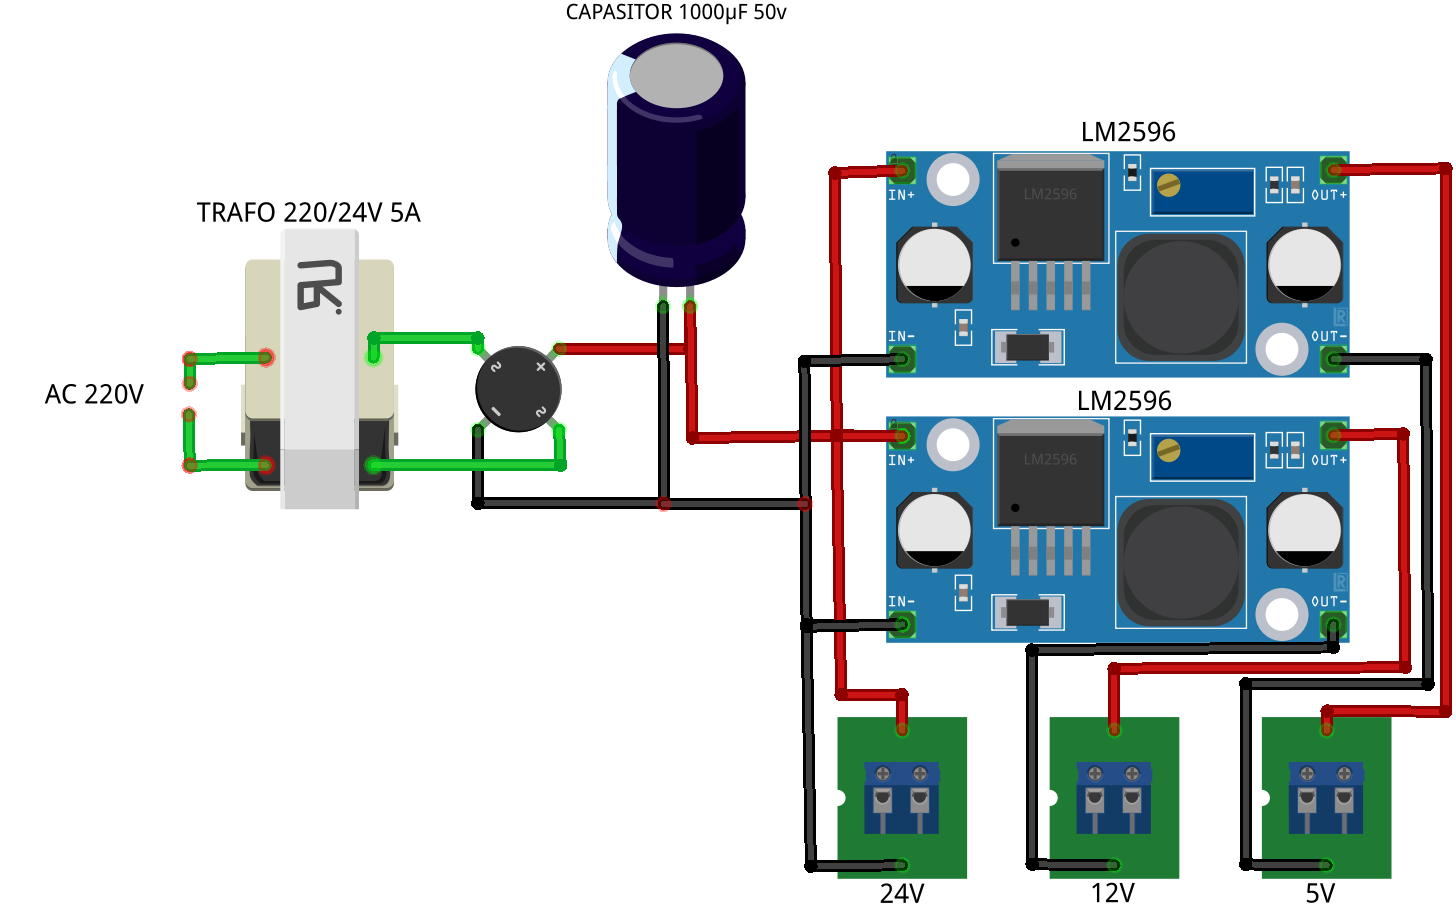
\includegraphics[width=8cm]{gambar/catudaya_bb.png}
	\caption{Sistem Secara Keseluruhan}
	\label{pic.sistemkeseluruhan}
\end{figure}

\begin{table}[H]
	\centering
	\caption{Keterangan Sistem Keseluruhan}
\label{tbl.sistemkeseluruhan}
		\begin{tabular}{|c|l|}
			\hline
			\rowcolor[HTML]{9B9B9B} 
			No & \multicolumn{1}{c|}{\cellcolor[HTML]{9B9B9B}Keterangan} \\ \hline
			1  & Robot Lengan SCARA                                      \\ \hline
			2  & Box Panel                                               \\ \hline
			3  & Arduino Mega 2560                                       \\ \hline
			4  & Personal Computer                                       \\ \hline
			5  & GUI Processing IDE                                      \\ \hline
			6  & Workspace Robot SCARA                                   \\ \hline
			7  & Kompresor                                               \\ \hline
			8  & Objek                                                   \\ \hline
		\end{tabular}

\end{table}
Processing IDE merupakan piranti yang digunakan sebagai masukan data. Masukan dari Processing IDE adalah hasil dari perhitungan kinematika maju dan atau kinematika balik yang dimasukkan melalui GUI. Objek berada dalam cakupan \textit{workspace} yang telah ditentukan luasnya yang ditinjau dari cangkupan dari \textit{end-effector}. GUI dari Processing IDE ini diproses menggunakan komputer personal.  

Processing IDE juga menampilan nilai derajat setiap \textit{joint}, koordinat $x$ dan $y$ dari \textit{end-effector}. Koordinat $x$ dan $y$ yang telah didapatkan dari processing IDE diolah dalam perhitungan kinematika balik sehingga dapat ditemukan nilai besar derajat sudut setiap \textit{joint}. Setelah nilai besar derajat sudut setiap \textit{joint} didapatkan, Processing IDE akan mengirimkan nilai-nilai tersebut ke Arduino IDE melewati komunikasi Serial. Arduino Mega 2560 mengirimkan nilai-nilai tersebut sesuai dengan pin motor DC yang tersambung dengan Arduino Mega 2560 melalui \textit{Driver} Motor H-\textit{Bridge} EMS 30A, kemudian nilai-nilai \textit{joint}  tersebut dikirimkan Arduino Mega 2560 kembali ke Processing IDE melalui koneksi langsung menggunakan kabel USB.  

Arduino Mega 2560 merupakan mikrokotroler yang menggerakkan setiap motor DC sesuai dengan besaran nilai yang telah didapatkan. Robot lengan SCARA akan mencapai koordinat $x$ dan $y$ dari objek, lalu mencengkram objek tersebut menggunakan \textit{Gripper}.
